\documentclass[11pt, a4paper]{article}
%\usepackage{proj1}
\usepackage{natbib}
\usepackage{fancyhdr}  
\usepackage{subcaption}
\usepackage{caption}
\usepackage{graphicx}
\linespread{1.25} 
\setlength{\parindent}{0cm}
\graphicspath{{Images/}}
\usepackage{hyperref}
\usepackage{amsmath}
\usepackage{amsfonts}
\usepackage{amssymb}
\usepackage{amsthm}
\usepackage{mathtools}
\usepackage{commath}

%\usepackage[sc,osf]{mathpazo}
\usepackage{subcaption}
\usepackage[a4paper, top=1in, left=1.0in, right=1.0in, bottom=1in, includehead, includefoot]{geometry} %Usually have top as 1in

\usepackage{listings}
\usepackage{color} %red, green, blue, yellow, cyan, magenta, black, white
\definecolor{mygreen}{RGB}{28,172,0} % color values Red, Green, Blue
\definecolor{mylilas}{RGB}{170,55,241}


\hypersetup{colorlinks,linkcolor={black},citecolor={blue},urlcolor={black}}
\usepackage{color}
\urlstyle{same}


\theoremstyle{definition}
\newtheorem{definition}{Definition}[section]

\title{Exact Solutions for the Full Problem \\with Force Control and with Flow Control}
\date{}
\newcommand{\Sta}{\rho}
\newcommand{\Adj}{p}
\newcommand{\Con}{u}

\pagenumbering{gobble}
\begin{document}
	
\section*{Report 07/05/2020}
Question: Plotting 2D Optimal Control?\\
Question: Running with Datastorage on the server (loading data).
\section{2D Examples}
All of the examples are done with FixPt, ODE Tols $= 10^{-8}$, Opti Tols $= 10^{-4}$ and $N1 \times N2 = 40 \times 40$, $n = 41$.
\subsection{Example 1: Neumann Flow Control, Symmetric}
The initial condition is:
\begin{align*}
\rho_{IC} = 0.5,
\end{align*}
and the target is:
\begin{align*}
\hat \rho = 0.5(1-t) + t\frac{1}{4}((\cos(\pi y_1)+2)(\cos(\pi y_2)+2)).
\end{align*}
When $\beta = 10^{-3}$, choose $\gamma = -0.3$ and $\gamma = 0.3$. Both converge within about $700$ to $800$ Iterations.
For $\gamma=0.3$, $J_{FW} = 0.3639$, $J_{Opt} = 0.1946$, see Figures \ref{Ex12DN1}, \ref{Ex12DN1a} and \ref{Ex12DN1b}.
\begin{figure}[h]
	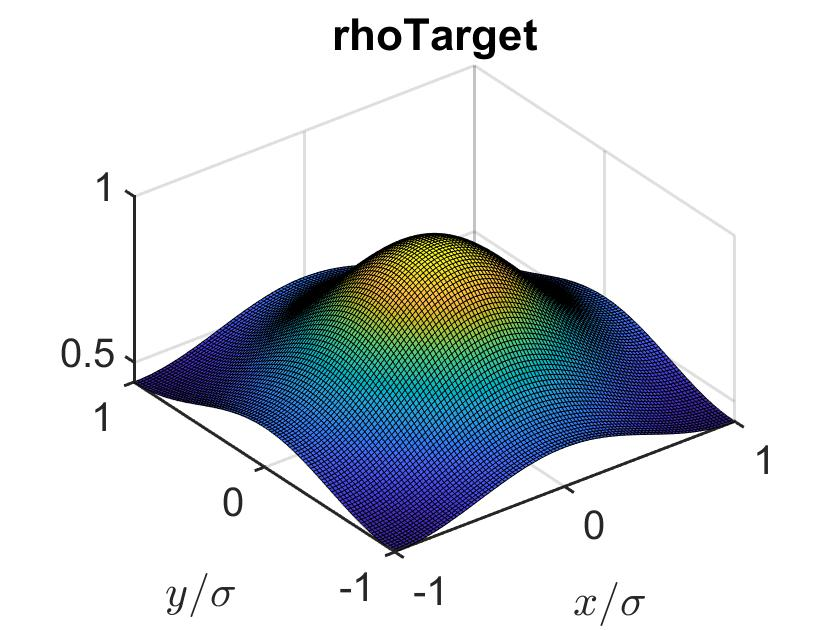
\includegraphics[scale=0.3]{rhoHat2DN1.jpg}
	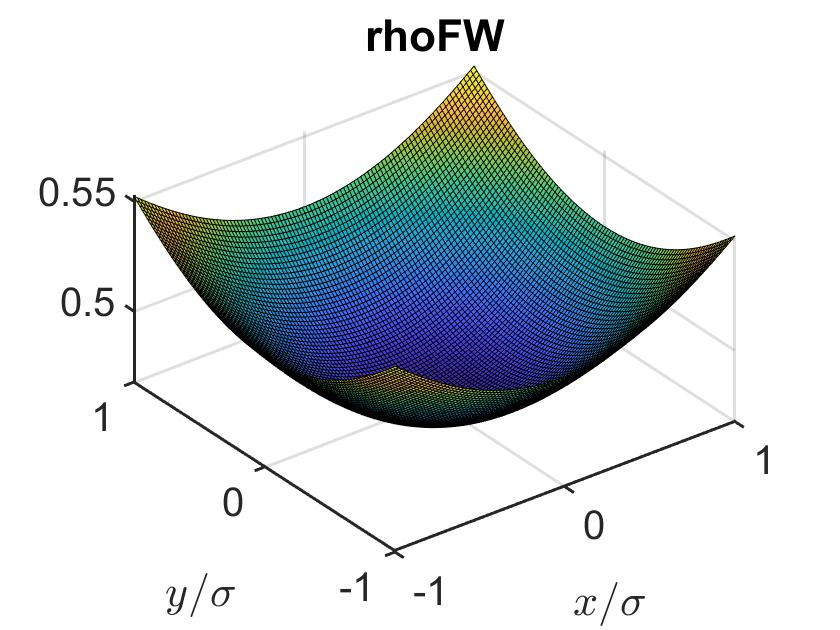
\includegraphics[scale=0.3]{rhoFW2DN1.jpg}
	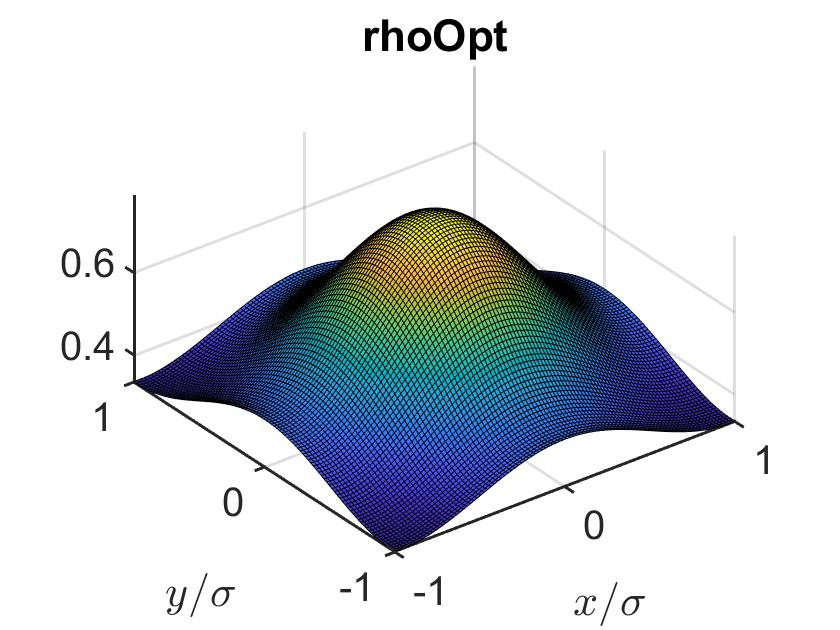
\includegraphics[scale=0.3]{rhoOpt2DN1.jpg}
	\caption{Results for Neumann Flow, Example 1 $\gamma = 0.3$, $t = 14/41$.}
	\label{Ex12DN1}
\end{figure}
\begin{figure}[h]
	\includegraphics[scale=0.3]{rhoHat2DN1a.jpg}
	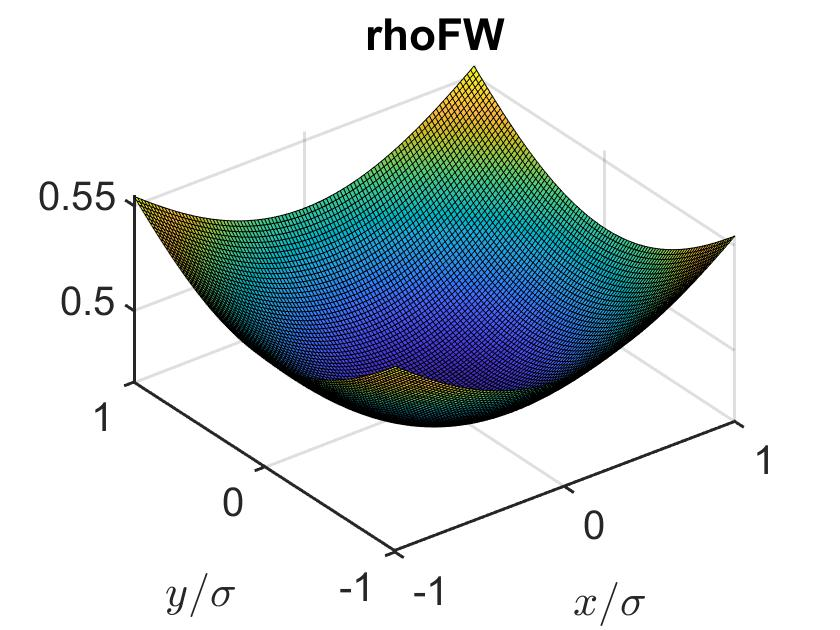
\includegraphics[scale=0.3]{rhoFW2DN1a.jpg}
	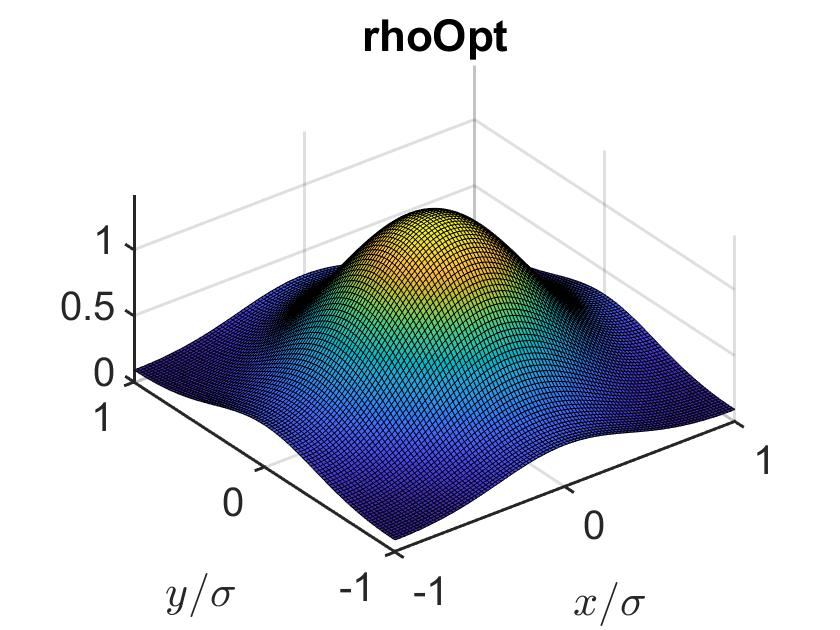
\includegraphics[scale=0.3]{rhoOpt2DN1a.jpg}
	\caption{Results for Neumann Flow, Example 1 $\gamma = 0.3$, $t = 28/41$.}
	\label{Ex12DN1a}
\end{figure}
\begin{figure}[h]
	\includegraphics[scale=0.3]{rhoHat2DN1b.jpg}
	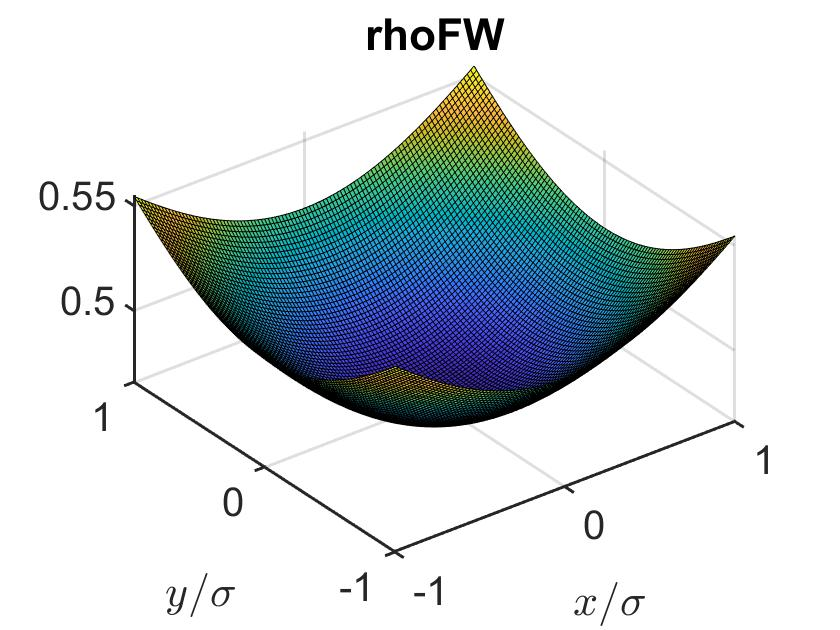
\includegraphics[scale=0.3]{rhoFW2DN1b.jpg}
	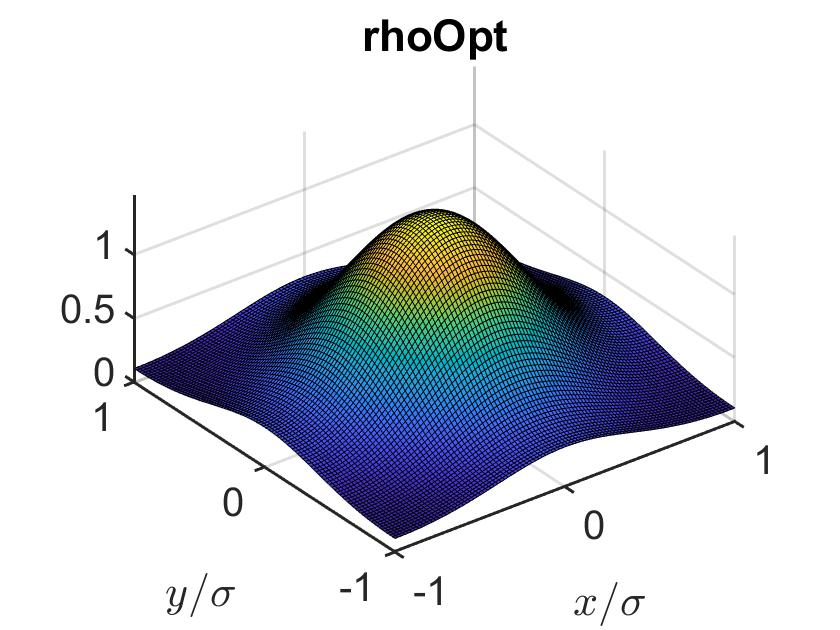
\includegraphics[scale=0.3]{rhoOpt2DN1b.jpg}
	\caption{Results for Neumann Flow, Example 1 $\gamma = 0.3$, $t = 41/41$.}
	\label{Ex12DN1b}
\end{figure}
For $\gamma= -0.3$, $J_{FW} =0.3111$, $J_{Opt} = 0.1733$, see Figures \ref{Ex12DN2}, \ref{Ex12DN2a} and \ref{Ex12DN2b}.
\begin{figure}[h]
	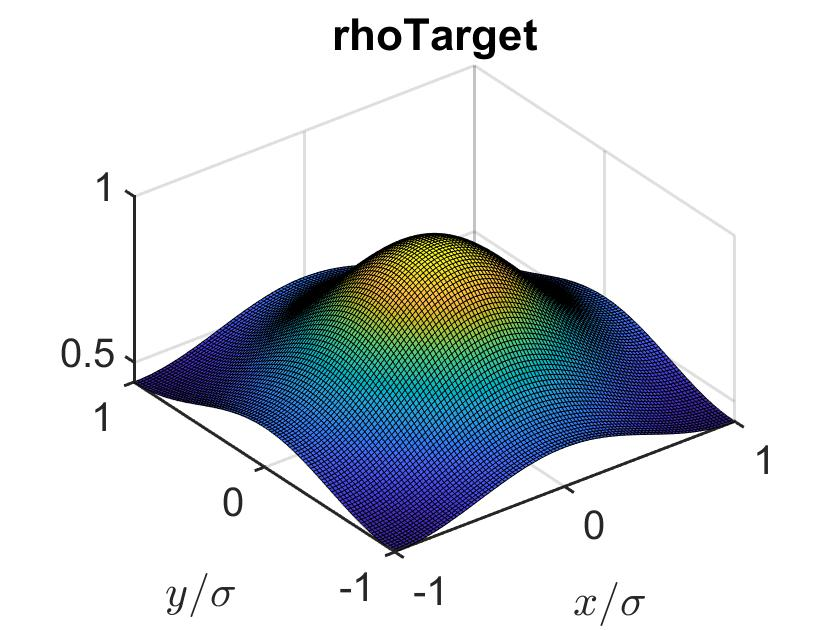
\includegraphics[scale=0.3]{rhoHat2DN2.jpg}
	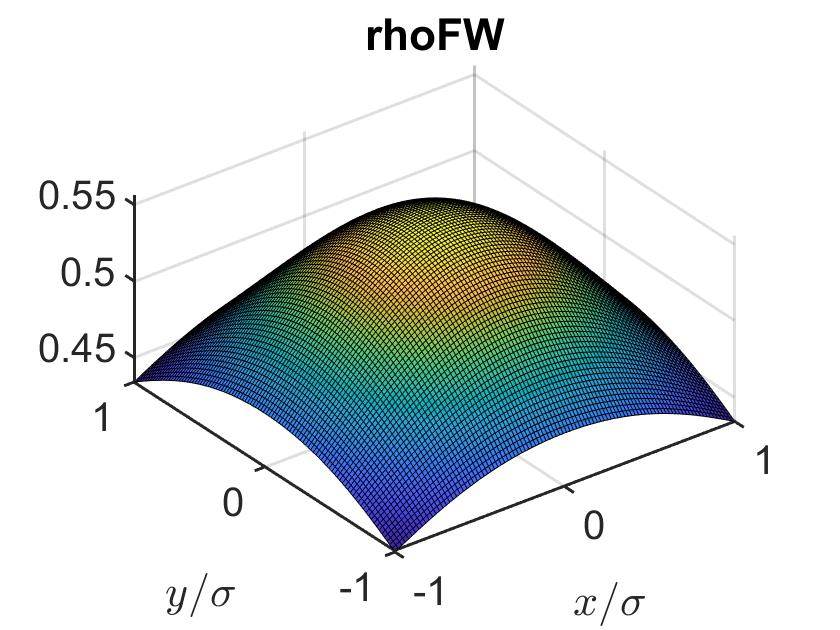
\includegraphics[scale=0.3]{rhoFW2DN2.jpg}
	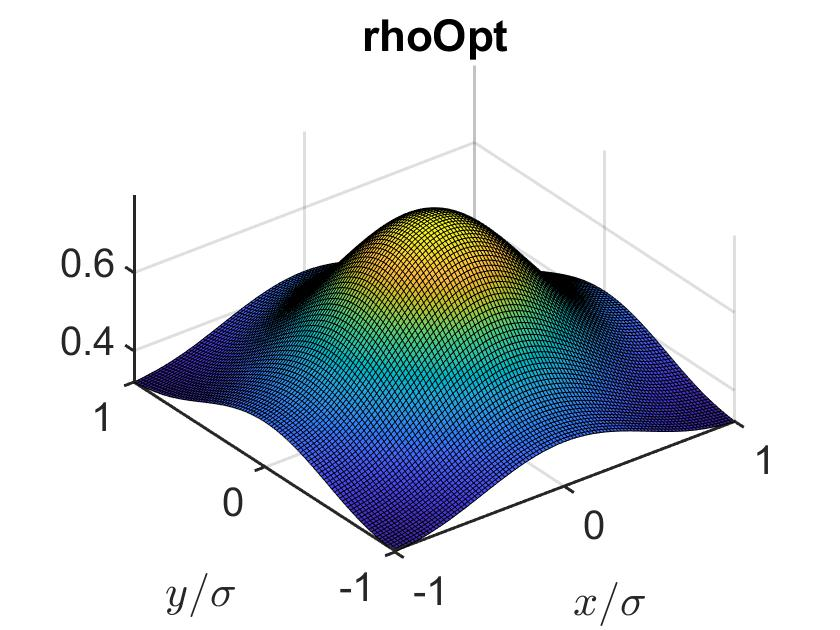
\includegraphics[scale=0.3]{rhoOpt2DN2.jpg}
	\caption{Results for Neumann Flow, Example 1 $\gamma = -0.3$, $t = 14/41$.}
	\label{Ex12DN2}
\end{figure}
\begin{figure}[h]
	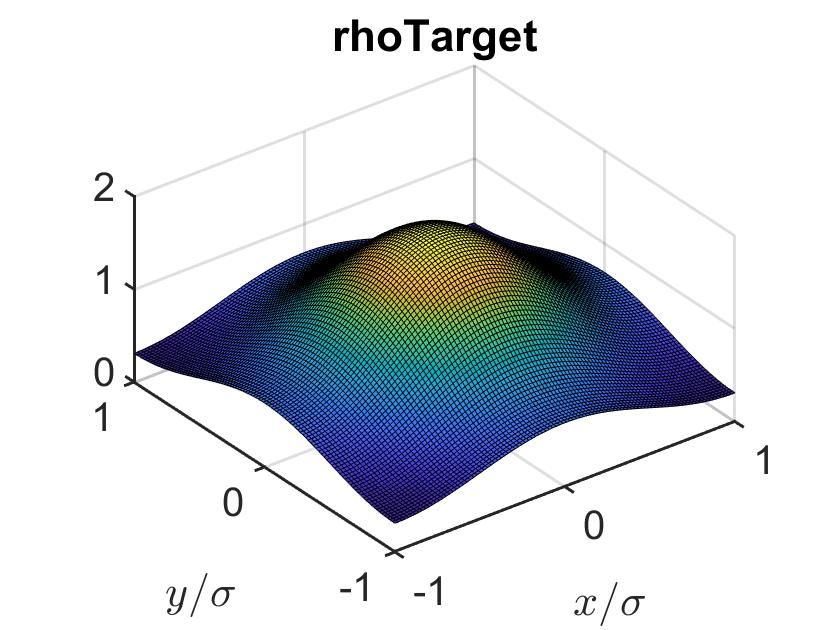
\includegraphics[scale=0.3]{rhoHat2DN2a.jpg}
	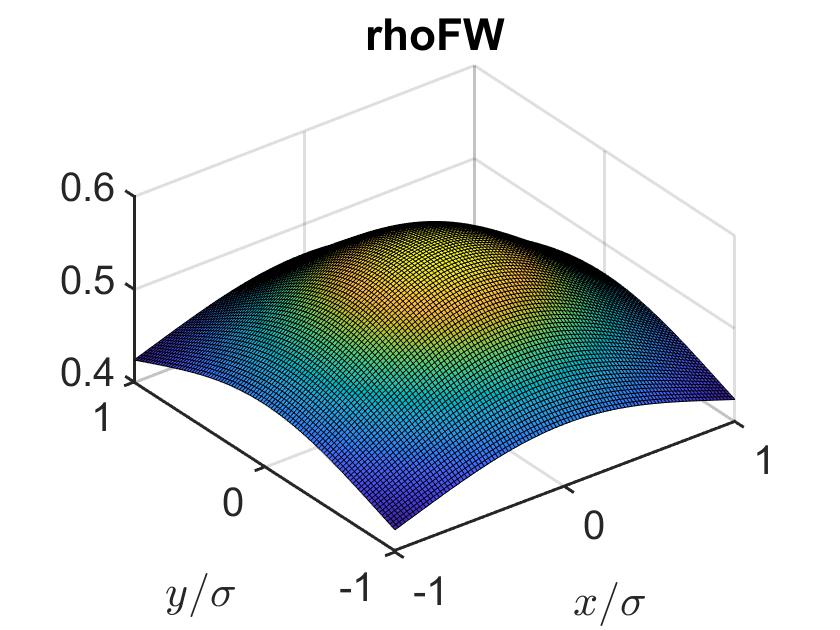
\includegraphics[scale=0.3]{rhoFW2DN2a.jpg}
	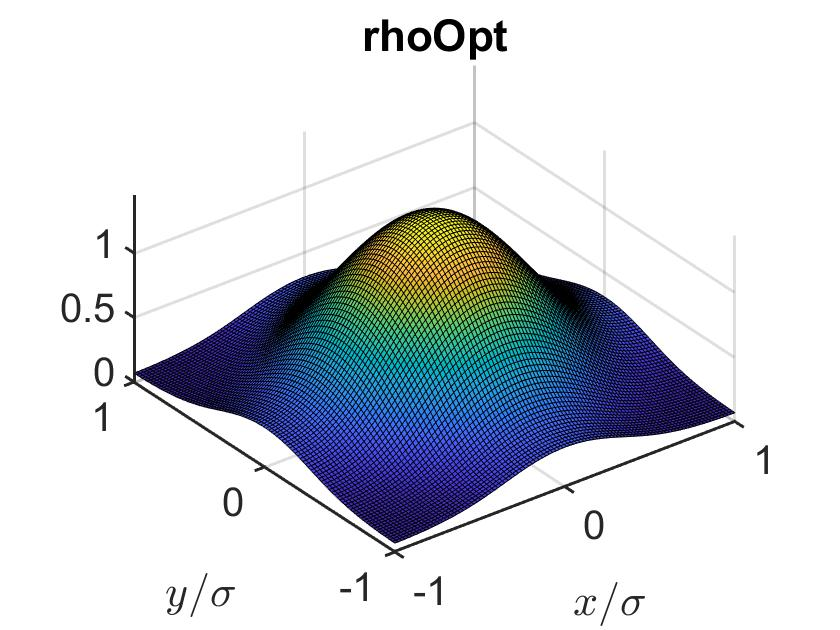
\includegraphics[scale=0.3]{rhoOpt2DN2a.jpg}
	\caption{Results for Neumann Flow, Example 1 $\gamma = -0.3$, $t = 28/41$.}
	\label{Ex12DN2a}
\end{figure}
\begin{figure}[h]
	\includegraphics[scale=0.3]{rhoHat2DN2b.jpg}
	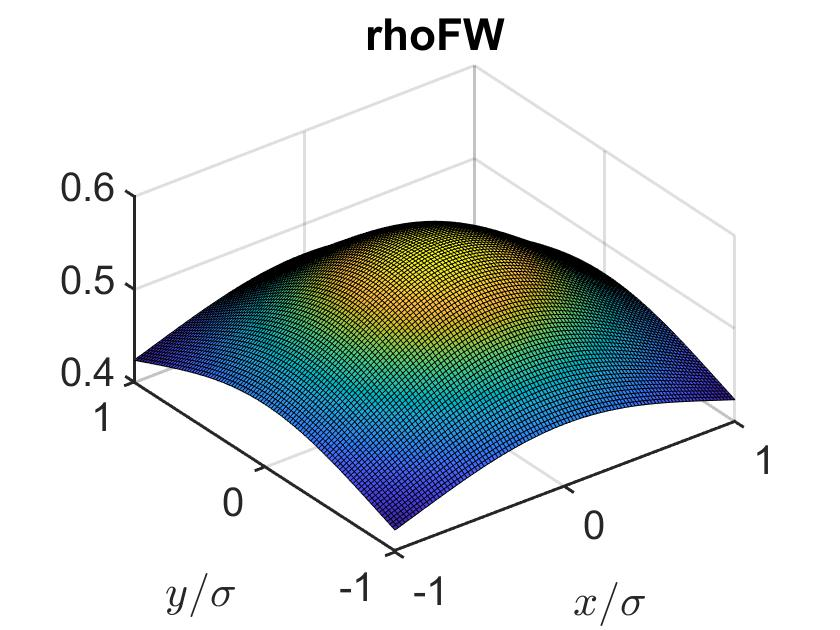
\includegraphics[scale=0.3]{rhoFW2DN2b.jpg}
	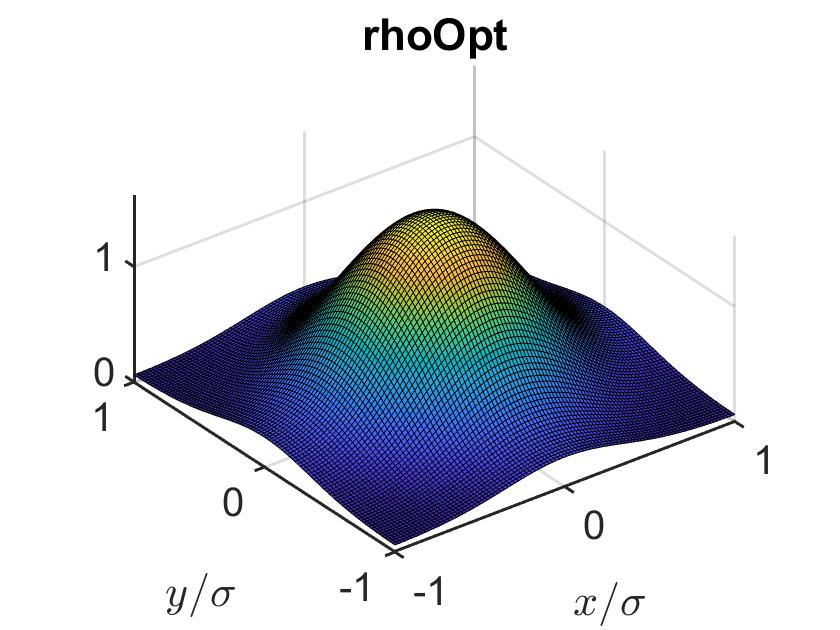
\includegraphics[scale=0.3]{rhoOpt2DN2b.jpg}
	\caption{Results for Neumann Flow, Example 1 $\gamma = -0.3$, $t = 41/41$.}
	\label{Ex12DN2b}
\end{figure}
\subsection{Example 2: Neumann Flow Control, Asymmetric}
The initial condition is:
\begin{align*}
\rho_{IC} = 0.5,
\end{align*}
and the target is:
\begin{align*}
\hat \rho = 0.5(1-t) + t\bigg(\frac{1}{2}((\sin(\pi (y_1 - 2)/2))\sin(\pi(y_2 - 2)/2)) + \frac{1}{2}\bigg).
\end{align*}
When $\beta = 10^{-3}$, choose $\gamma = -0.3$ and $\gamma = 0.3$. Both converge within about $700$ to $800$ Iterations.
For $\gamma = 0.3$, $J_{FW} = 0.0424$, $J_{Opt} = 0.0025$, see Figures \ref{Ex12DN3}, \ref{Ex12DN3a}, \ref{Ex12DN3b}
\begin{figure}[h]
	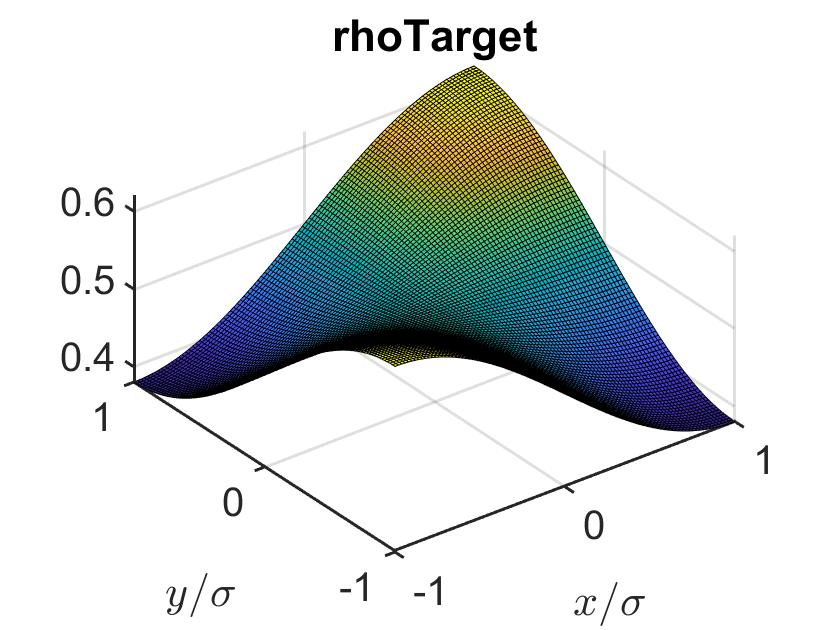
\includegraphics[scale=0.3]{rhoHat2DN3.jpg}
	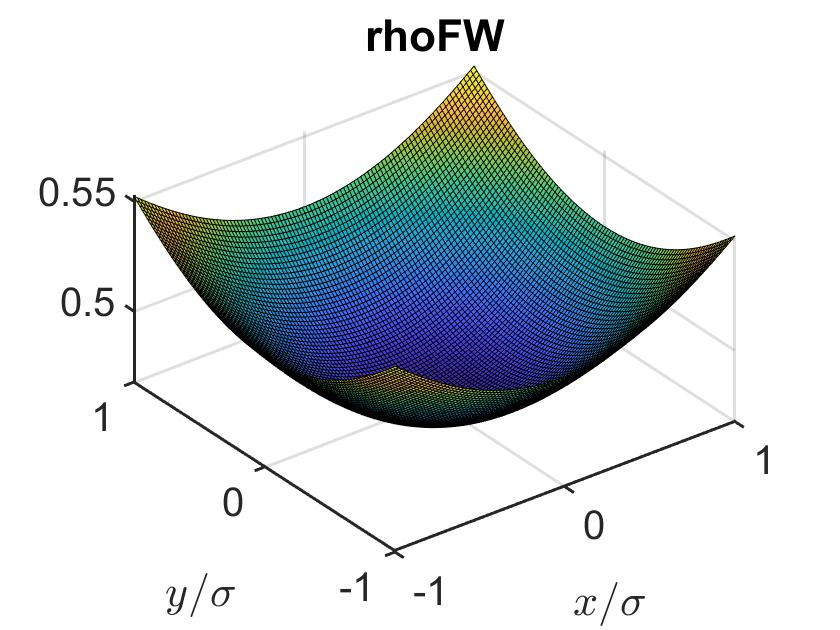
\includegraphics[scale=0.3]{rhoFW2DN3.jpg}
	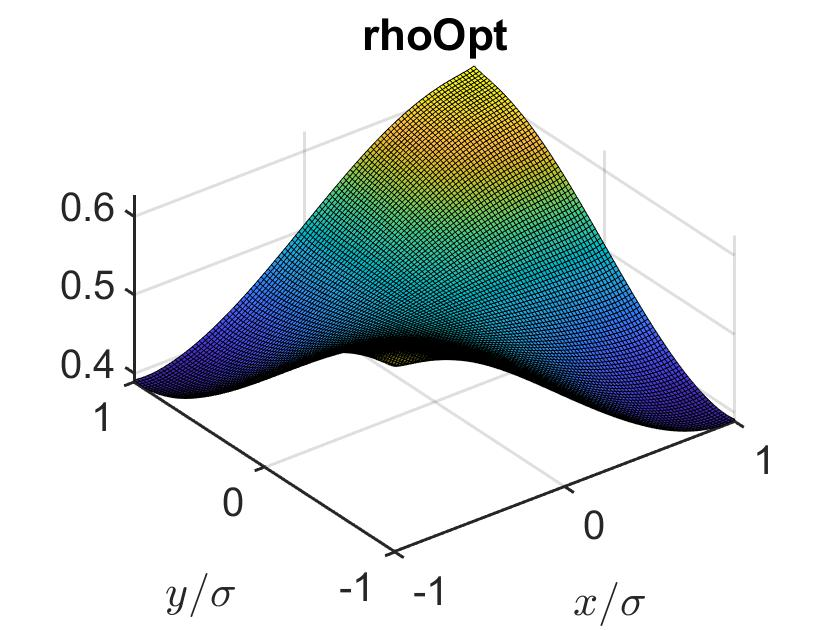
\includegraphics[scale=0.3]{rhoOpt2D3.jpg}
	\caption{Results for Neumann Flow, Example 2 $\gamma = 0.3$, $t = 14/41$.}
	\label{Ex12DN3}
\end{figure}
\begin{figure}[h]
	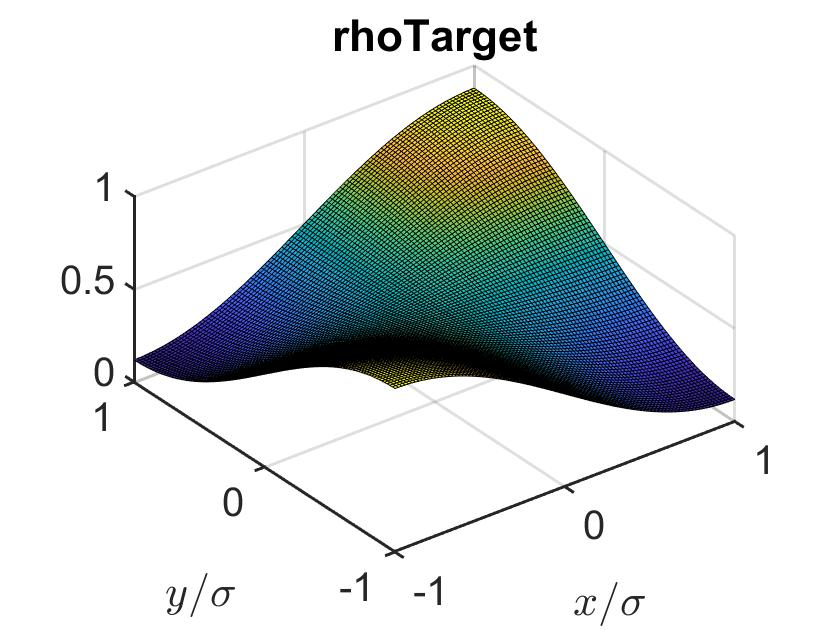
\includegraphics[scale=0.3]{rhoHat2DN3a.jpg}
	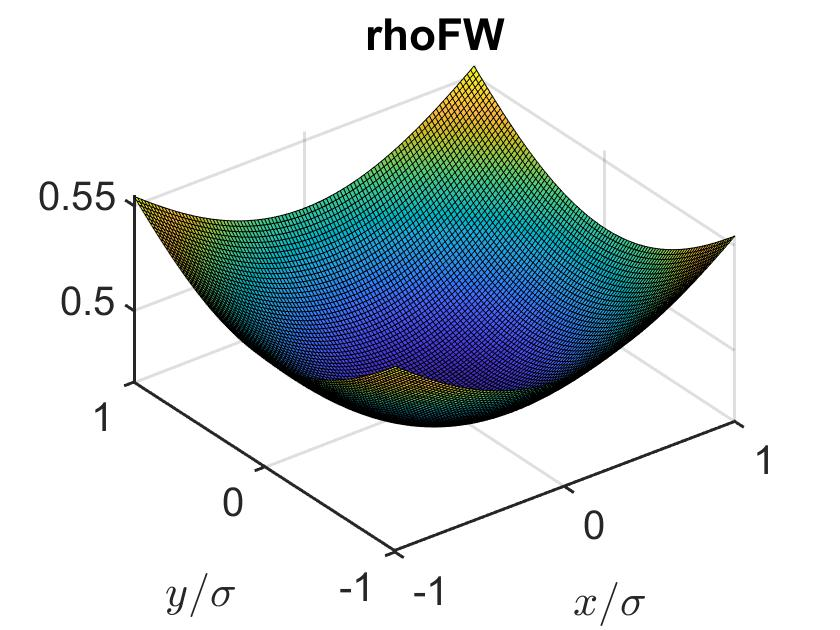
\includegraphics[scale=0.3]{rhoFW2DN3a.jpg}
	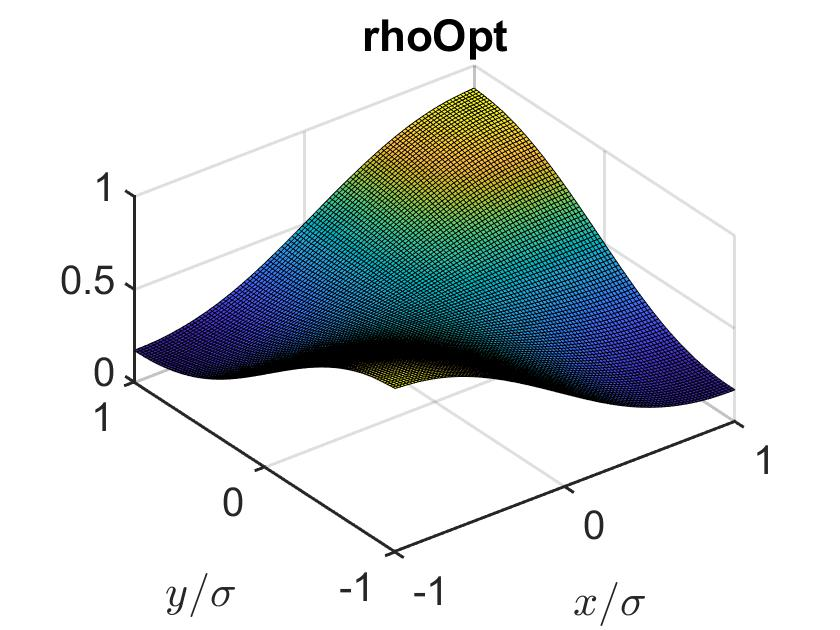
\includegraphics[scale=0.3]{rhoOpt2D3a.jpg}
	\caption{Results for Neumann Flow, Example 2 $\gamma = 0.3$, $t = 28/41$.}
	\label{Ex12DN3a}
\end{figure}
\begin{figure}[h]
	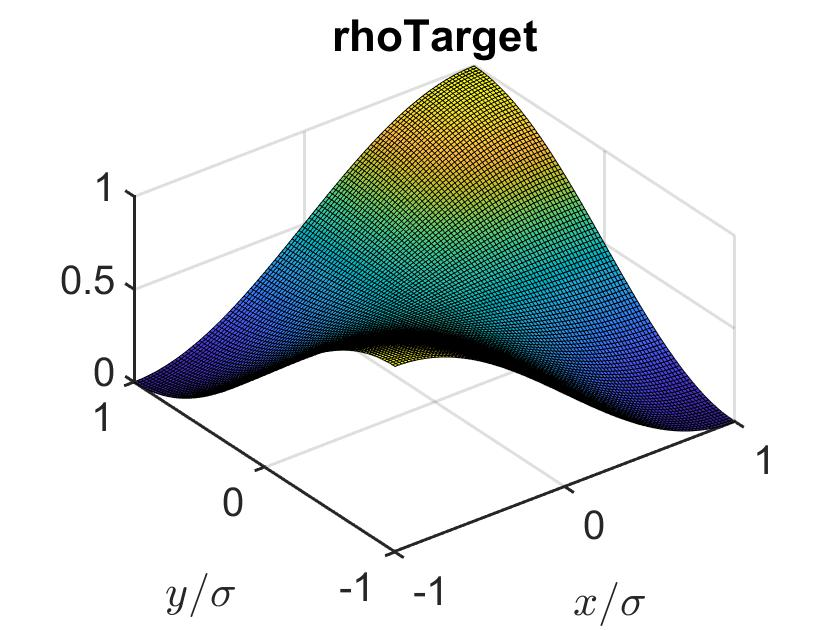
\includegraphics[scale=0.3]{rhoHat2DN3b.jpg}
	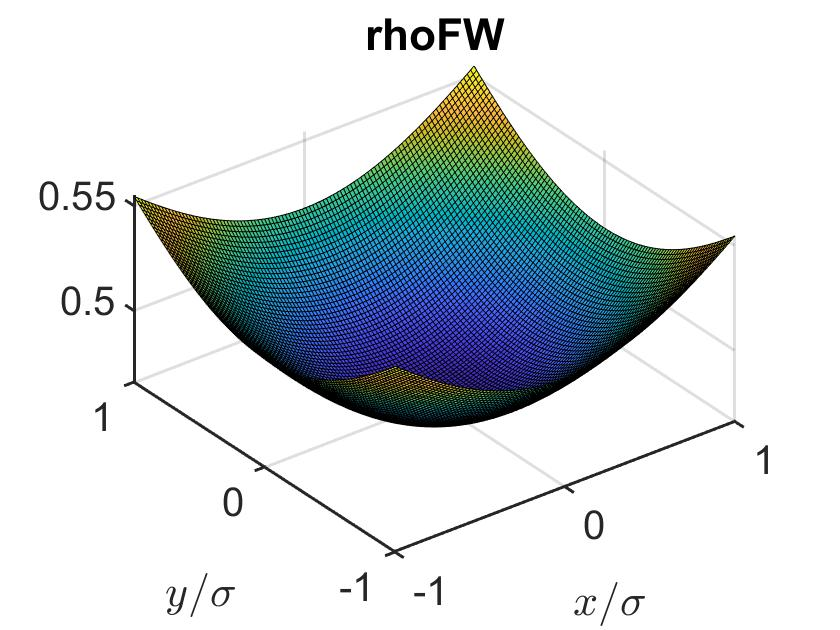
\includegraphics[scale=0.3]{rhoFW2DN3b.jpg}
	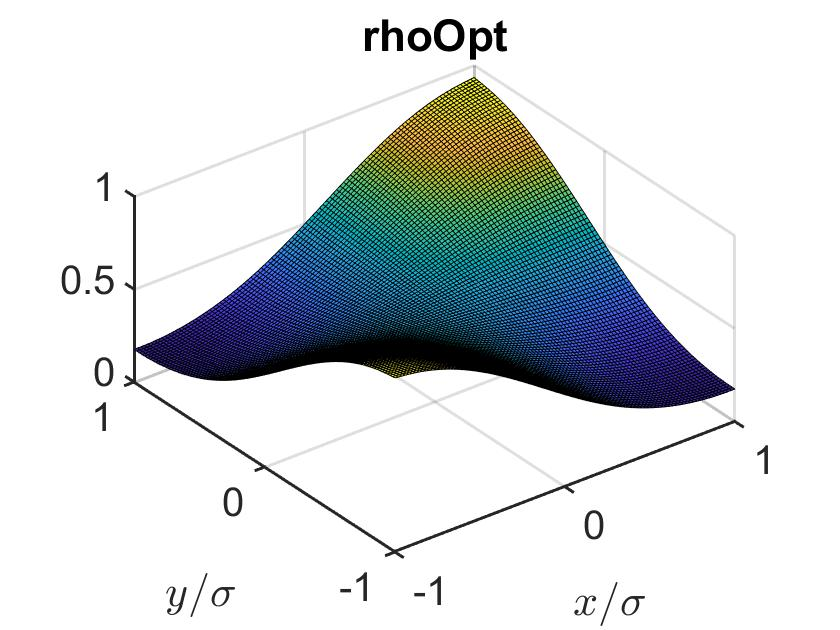
\includegraphics[scale=0.3]{rhoOpt2D3b.jpg}
	\caption{Results for Neumann Flow, Example 2 $\gamma = 0.3$, $t = 41/41$.}
	\label{Ex12DN3b}
\end{figure}
For $\gamma = -0.3$, $J_{FW} = 0.0437$, $J_{Opt} = 0.0011$, see Figures \ref{Ex12DN4}, \ref{Ex12DN4a} and \ref{Ex12DN4b}.
\begin{figure}[h]
	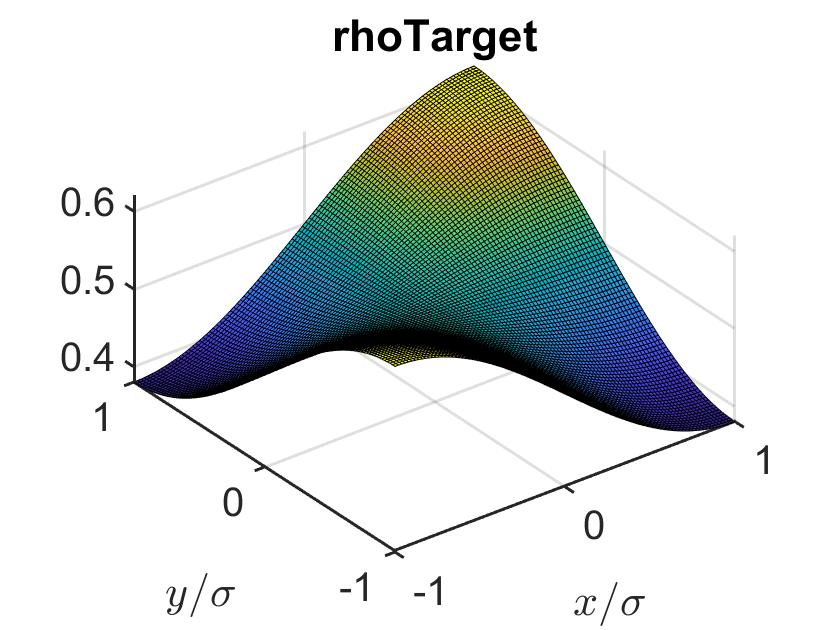
\includegraphics[scale=0.3]{rhoHat2DN4.jpg}
	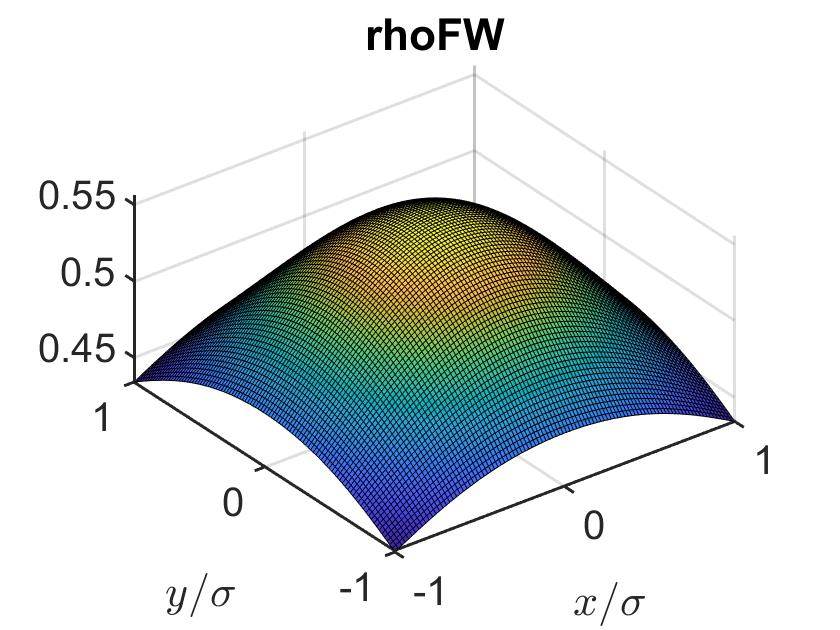
\includegraphics[scale=0.3]{rhoFW2DN4a.jpg}
	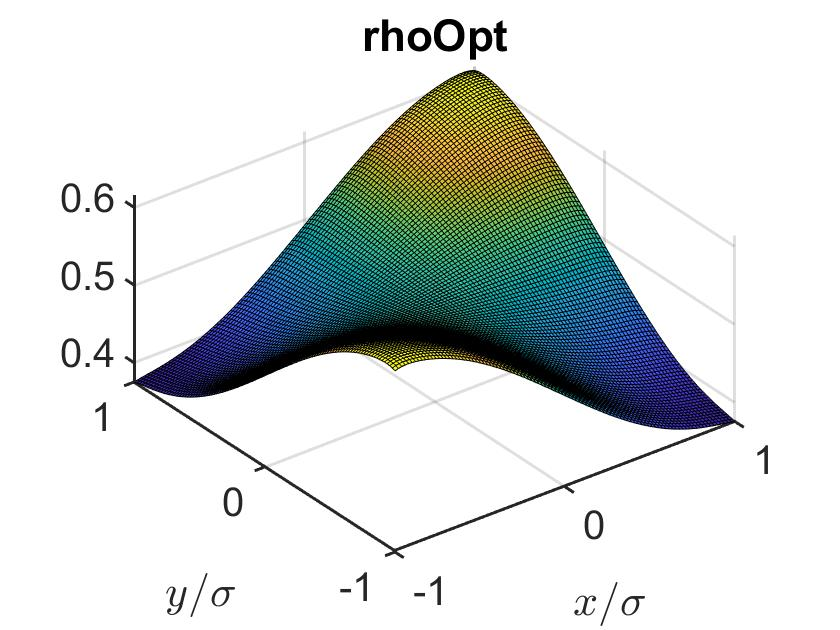
\includegraphics[scale=0.3]{rhoOpt2D4.jpg}
	\caption{Results for Neumann Flow, Example 2 $\gamma = -0.3$, $t = 14/41$.}
	\label{Ex12DN4}
\end{figure}
\begin{figure}[h]
	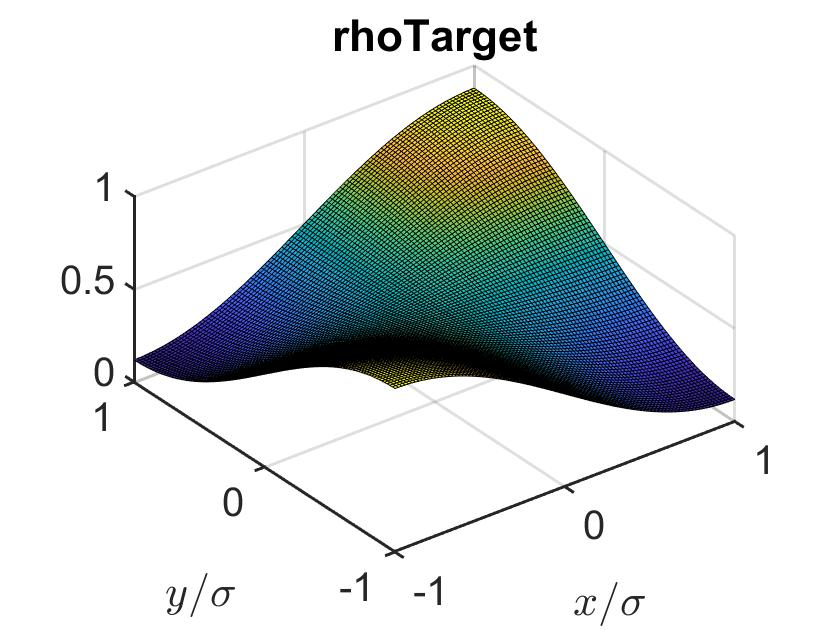
\includegraphics[scale=0.3]{rhoHat2DN4a.jpg}
	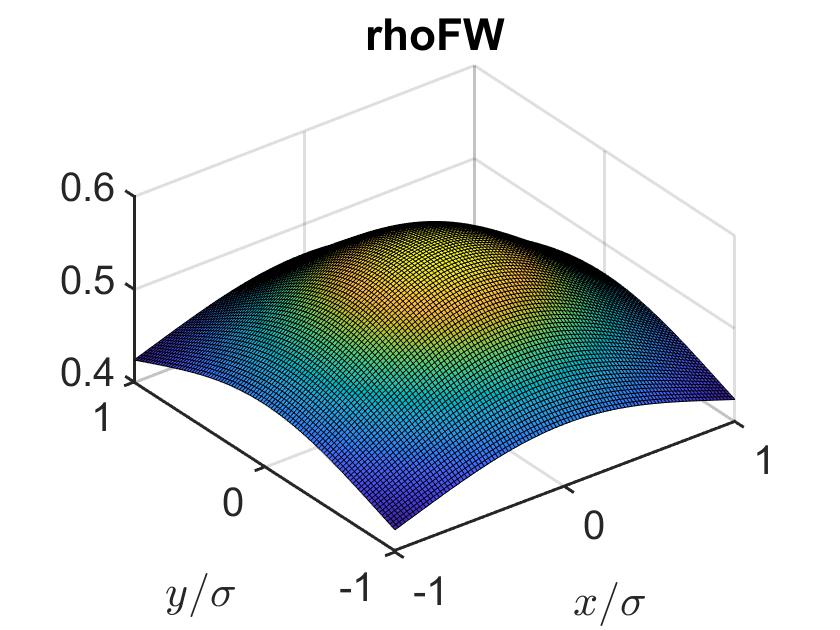
\includegraphics[scale=0.3]{rhoFW2DN4aa.jpg}
	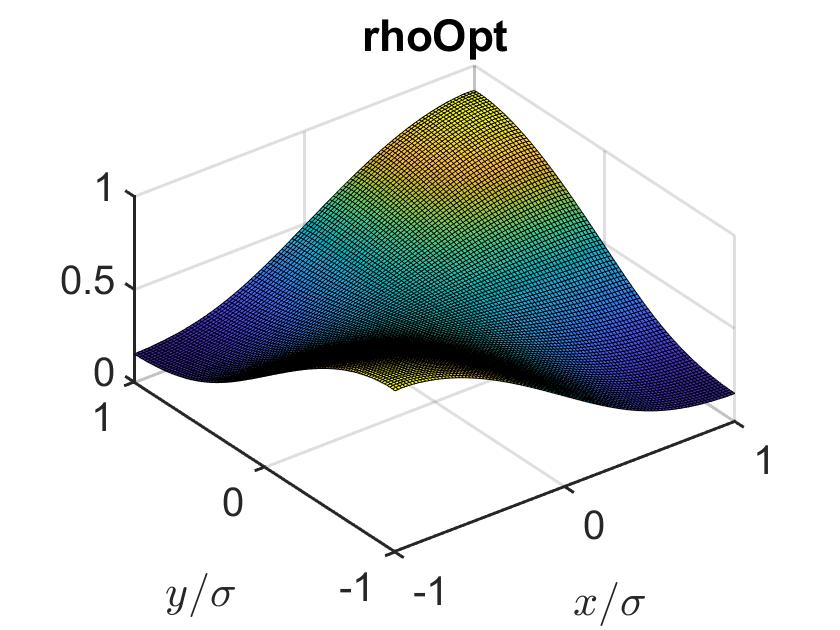
\includegraphics[scale=0.3]{rhoOpt2D4a.jpg}
	\caption{Results for Neumann Flow, Example 2 $\gamma = -0.3$, $t = 28/41$.}
	\label{Ex12DN4a}
\end{figure}
\begin{figure}[h]
	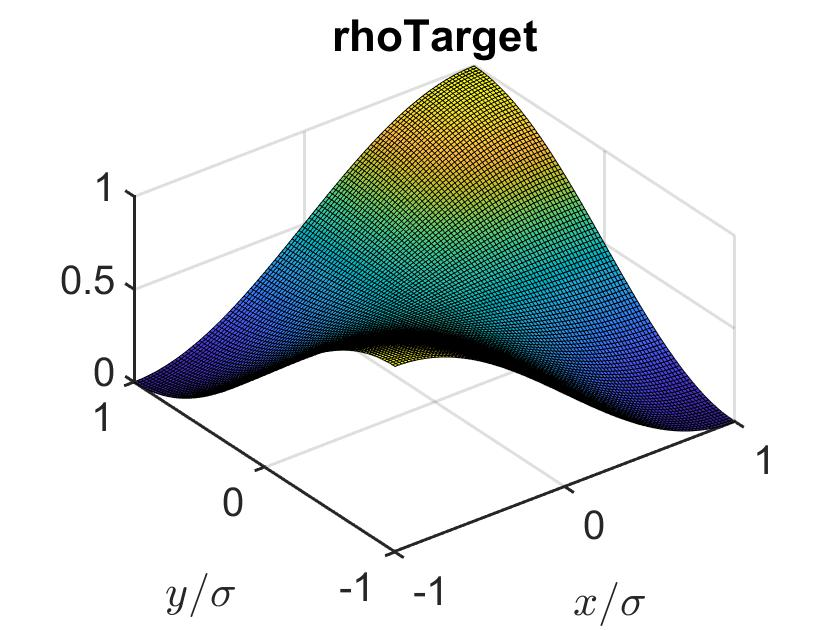
\includegraphics[scale=0.3]{rhoHat2DN4b.jpg}
	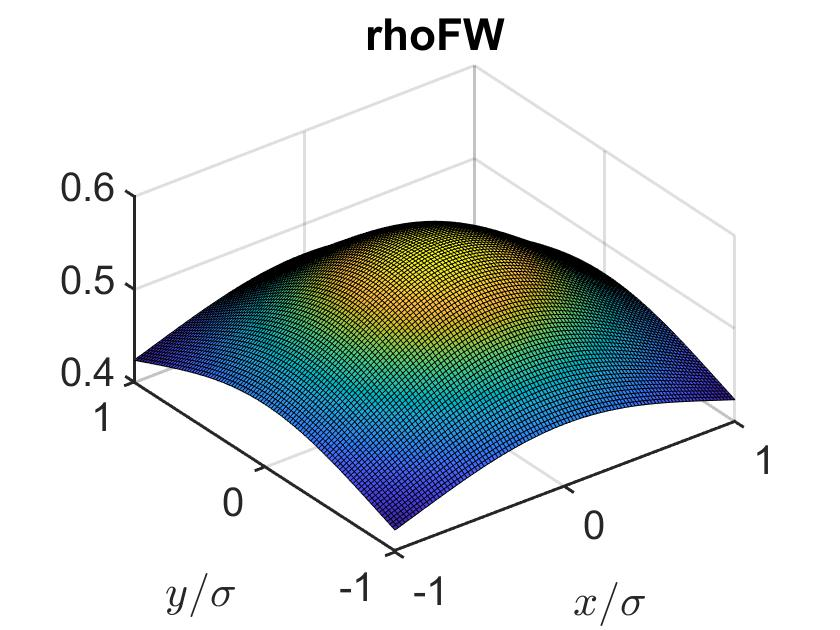
\includegraphics[scale=0.3]{rhoFW2DN4b.jpg}
	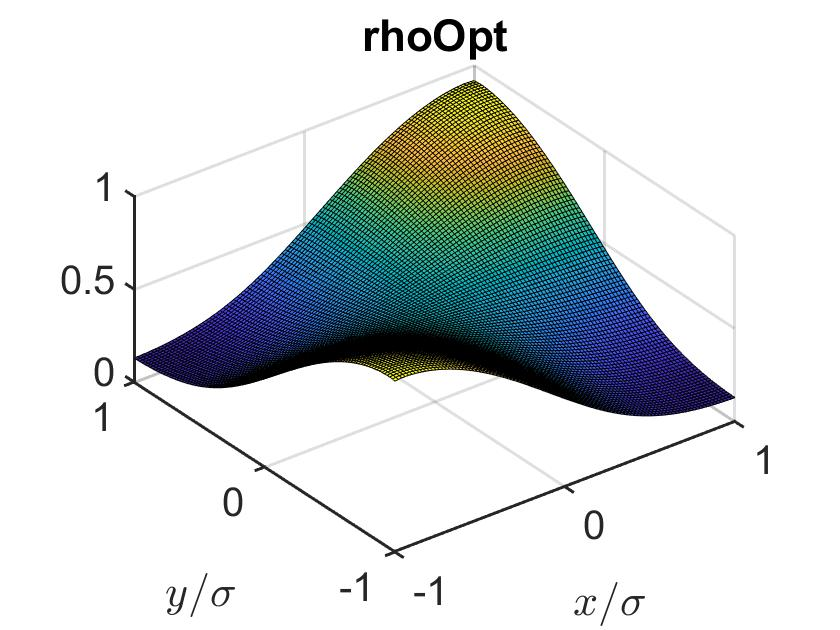
\includegraphics[scale=0.3]{rhoOpt2D4b.jpg}
	\caption{Results for Neumann Flow, Example 2 $\gamma = -0.3$, $t = 41/41$.}
	\label{Ex12DN4b}
\end{figure}
Both $\gamma = -0.3$ and $\gamma = 0.3$ converge for $\beta = 10$. $\rho_{Opt}$ is very close to $\rho_{FW}$ as expected.


\section{Two Peaks 1D Examples}
\subsection{Example 1}
Choose the intital condition:
\begin{align*}
\rho_{IC} = 0.5,
\end{align*}
and the target:
\begin{align*}
\hat \rho = 0.5(1-t) + t\bigg(\frac{1}{2}\cos(2 \pi y + \pi) + \frac{1}{2}\bigg).
\end{align*}
When $\gamma = 0$ and $\beta = 10^{-3}$, $J_{FW} = 0.0417$, $J_{Opt} = 0.0071$, see Figure \ref{Ex12Peak1}.
\begin{figure}[h]
	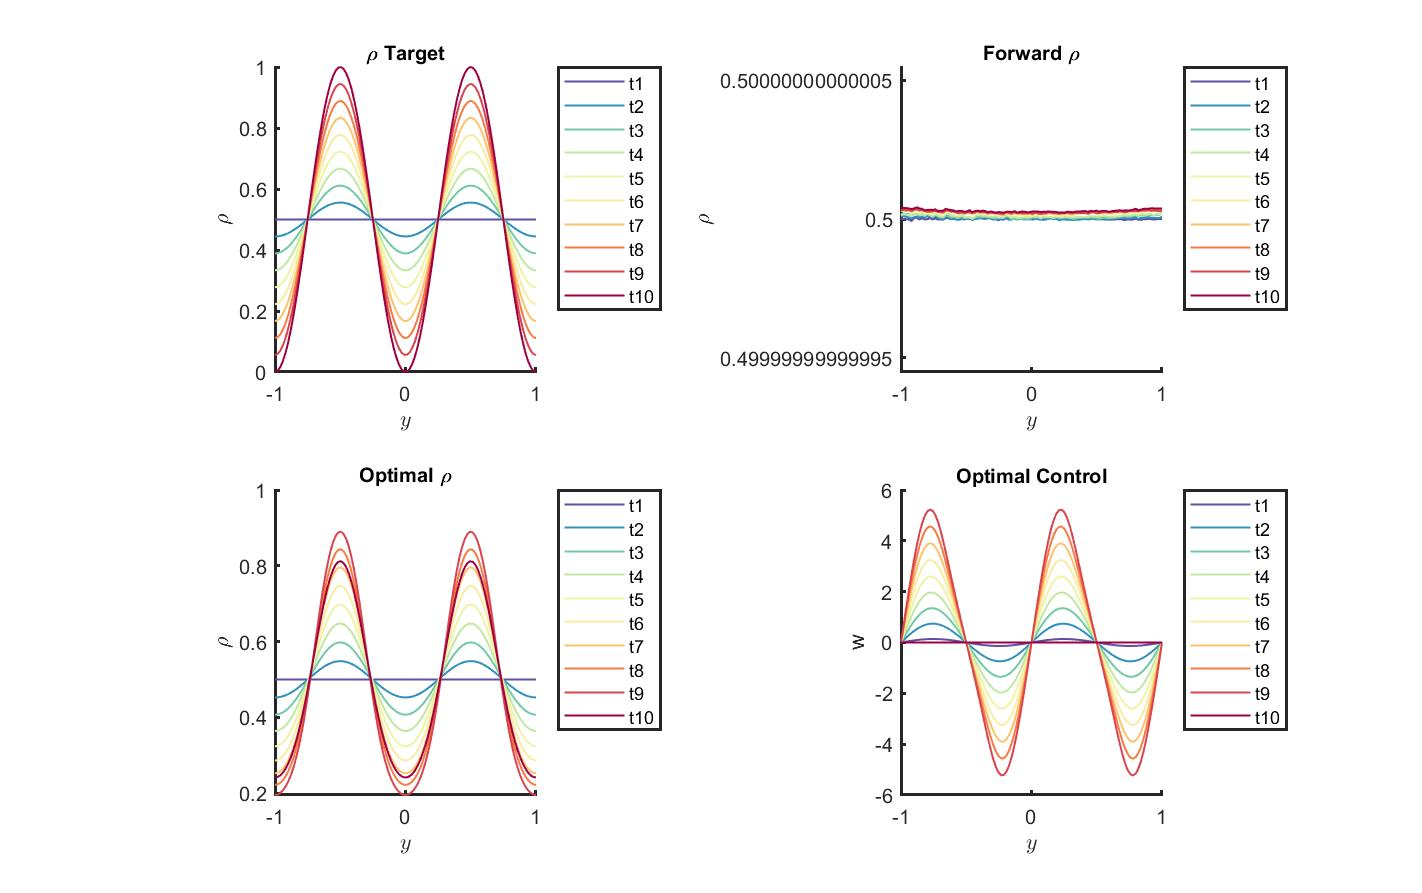
\includegraphics[scale=0.3]{Res2Peak1.jpg}
	\caption{Results for Neumann Flow, $2$ Peak Example $1$, $\gamma = 0$.}
	\label{Ex12Peak1}
\end{figure}
When $\gamma = -1$ and $\beta = 10^{-3}$, $J_{FW} = 0.0410$, $J_{Opt} = 0.0067$, see Figure \ref{Ex12Peak1a}.
\begin{figure}[h]
	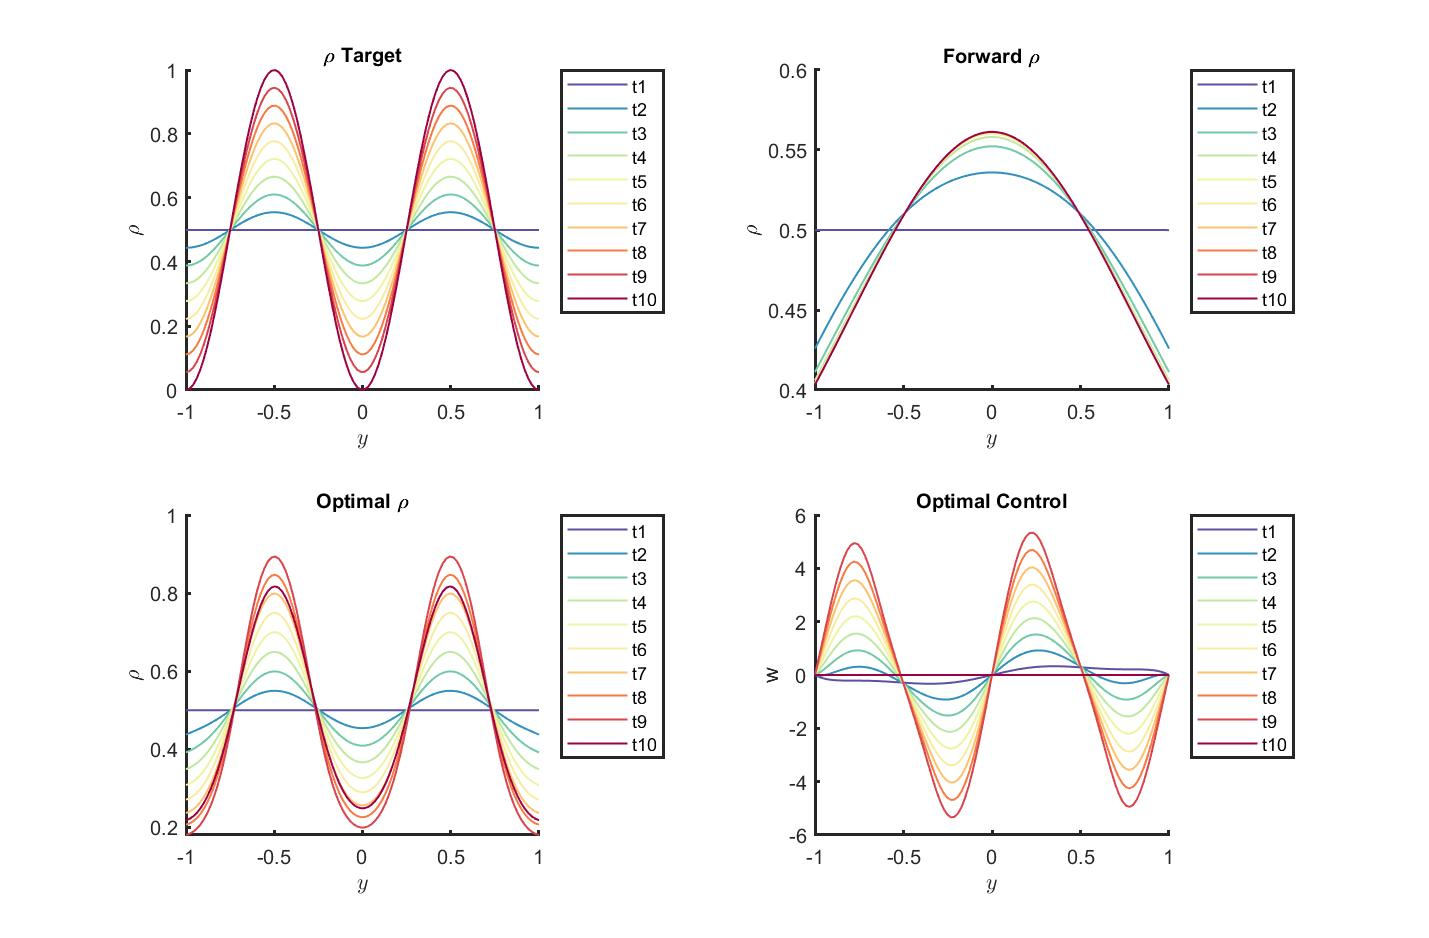
\includegraphics[scale=0.3]{Res2Peak1a.jpg}
	\caption{Results for Neumann Flow, $2$ Peak Example $1$, $\gamma = -1$.}
	\label{Ex12Peak1a}
\end{figure}
When $\gamma = 1$ and $\beta = 10^{-3}$, $J_{FW} = 0.0471$, $J_{Opt} = 0.0077$, see Figure \ref{Ex12Peak1b}.
\begin{figure}[h]
	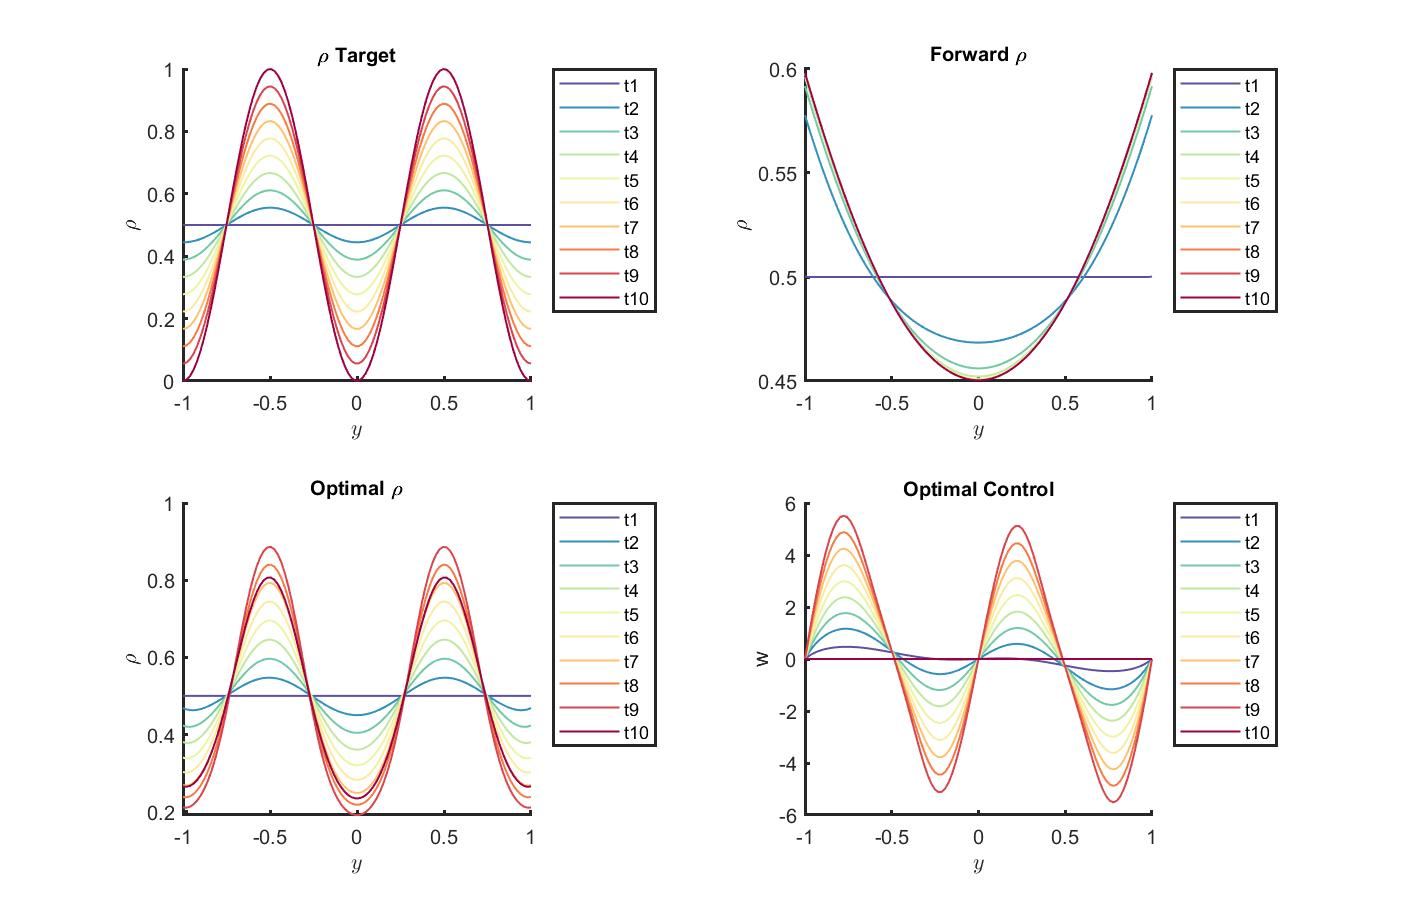
\includegraphics[scale=0.3]{Res2Peak1b.jpg}
	\caption{Results for Neumann Flow, $2$ Peak Example $1$, $\gamma = 1$.}
	\label{Ex12Peak1b}
\end{figure}

\subsection{Example 2}
Choose the intital condition:
\begin{align*}
\rho_{IC} = \frac{1}{2}\cos(\pi y) + \frac{1}{2},
\end{align*}
and the target:
\begin{align*}
\hat \rho = \bigg(\frac{1}{2}\cos(\pi y) + \frac{1}{2}\bigg)(1-t) + t\bigg(-\frac{1}{2}\cos(2 \pi y) + \frac{1}{2}\bigg).
\end{align*}
When $\gamma = 0$ and $\beta = 10^{-3}$, $J_{FW} = 0.0669$, $J_{Opt} = 0.0109$, see Figure \ref{Ex12Peak2}.
\begin{figure}[h]
	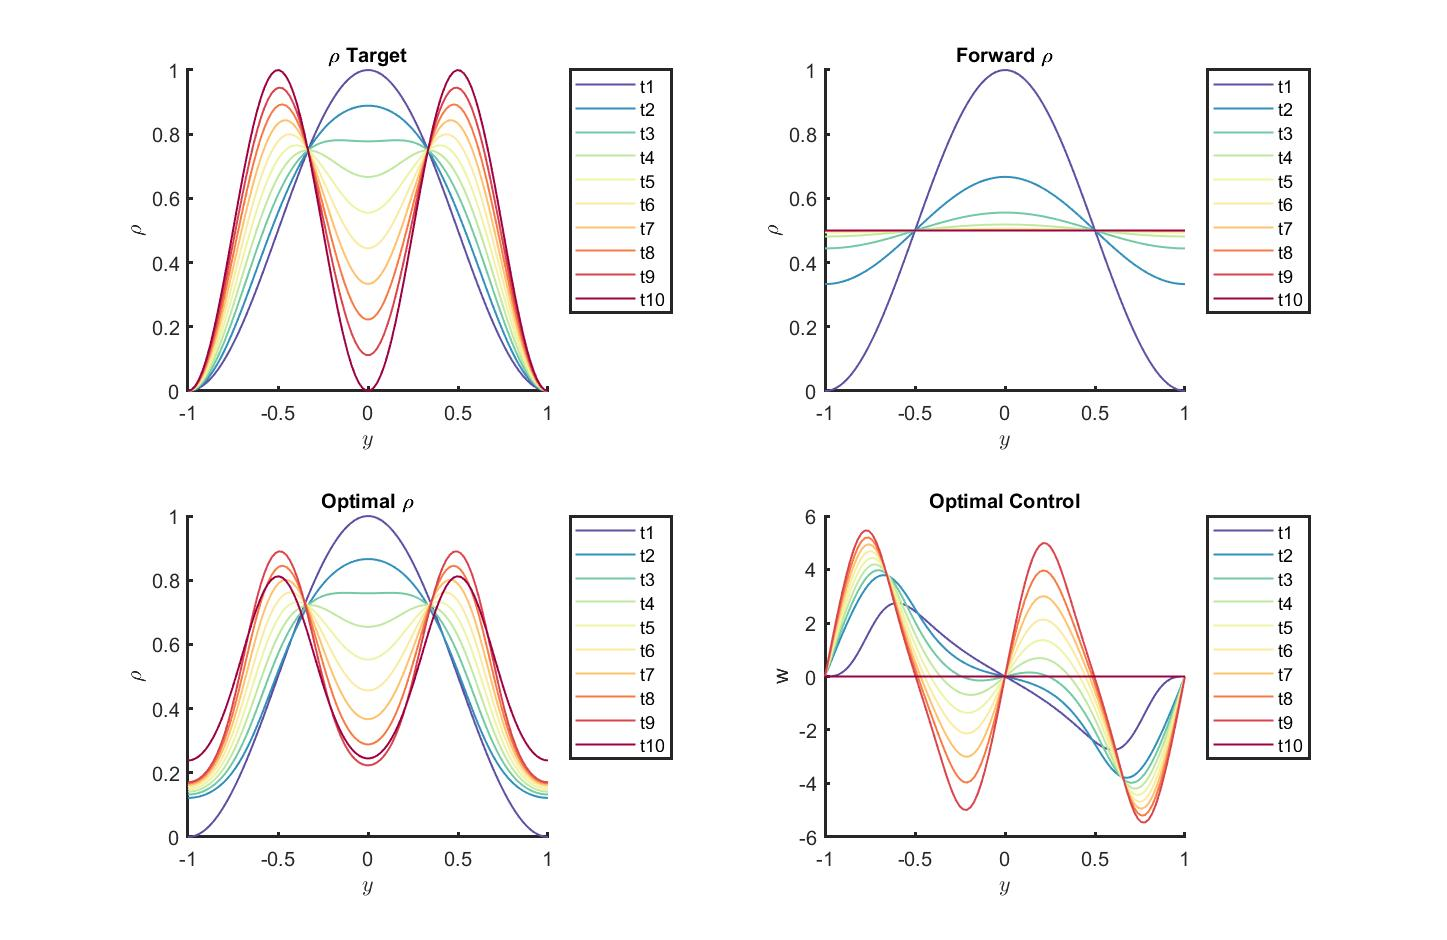
\includegraphics[scale=0.3]{Res2Peak2.jpg}
	\caption{Results for Neumann Flow, $2$ Peak Example $2$, $\gamma = 0$.}
	\label{Ex12Peak2}
\end{figure}
When $\gamma = -1$ and $\beta = 10^{-3}$, $J_{FW} = 0.05356$, $J_{Opt} = 0.0097$, see Figure \ref{Ex12Peak2a}.
\begin{figure}[h]
	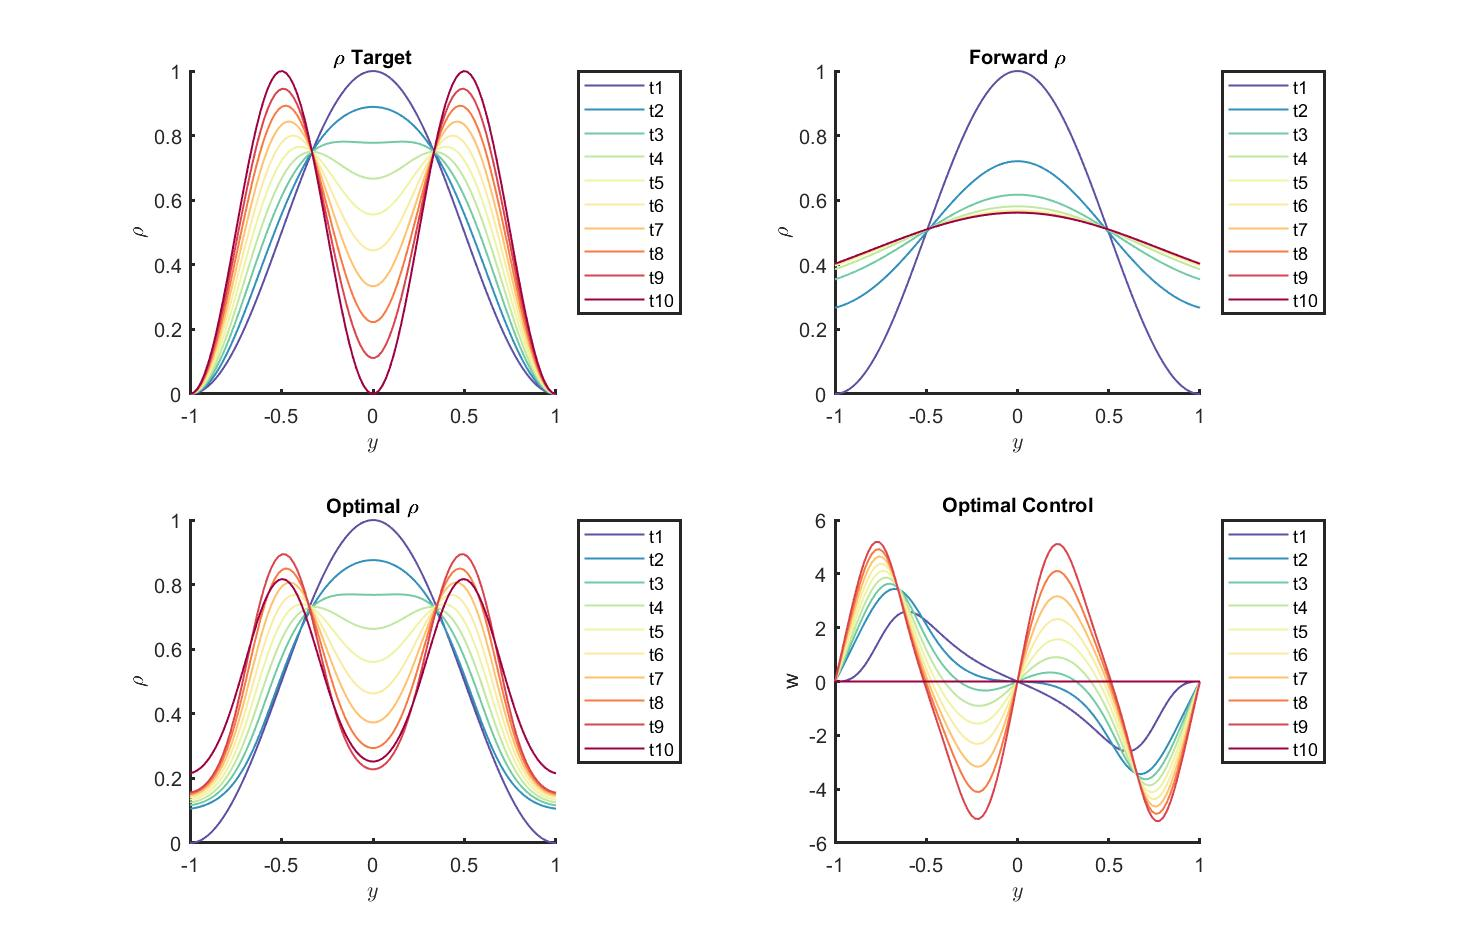
\includegraphics[scale=0.3]{Res2Peak2a.jpg}
	\caption{Results for Neumann Flow, $2$ Peak Example $2$, $\gamma = -1$.}
	\label{Ex12Peak2a}
\end{figure}
When $\gamma = 1$ and $\beta = 10^{-3}$, $J_{FW} = 0.0839$, $J_{Opt} = 0.0125$, see Figure \ref{Ex12Peak2b}.
\begin{figure}[h]
	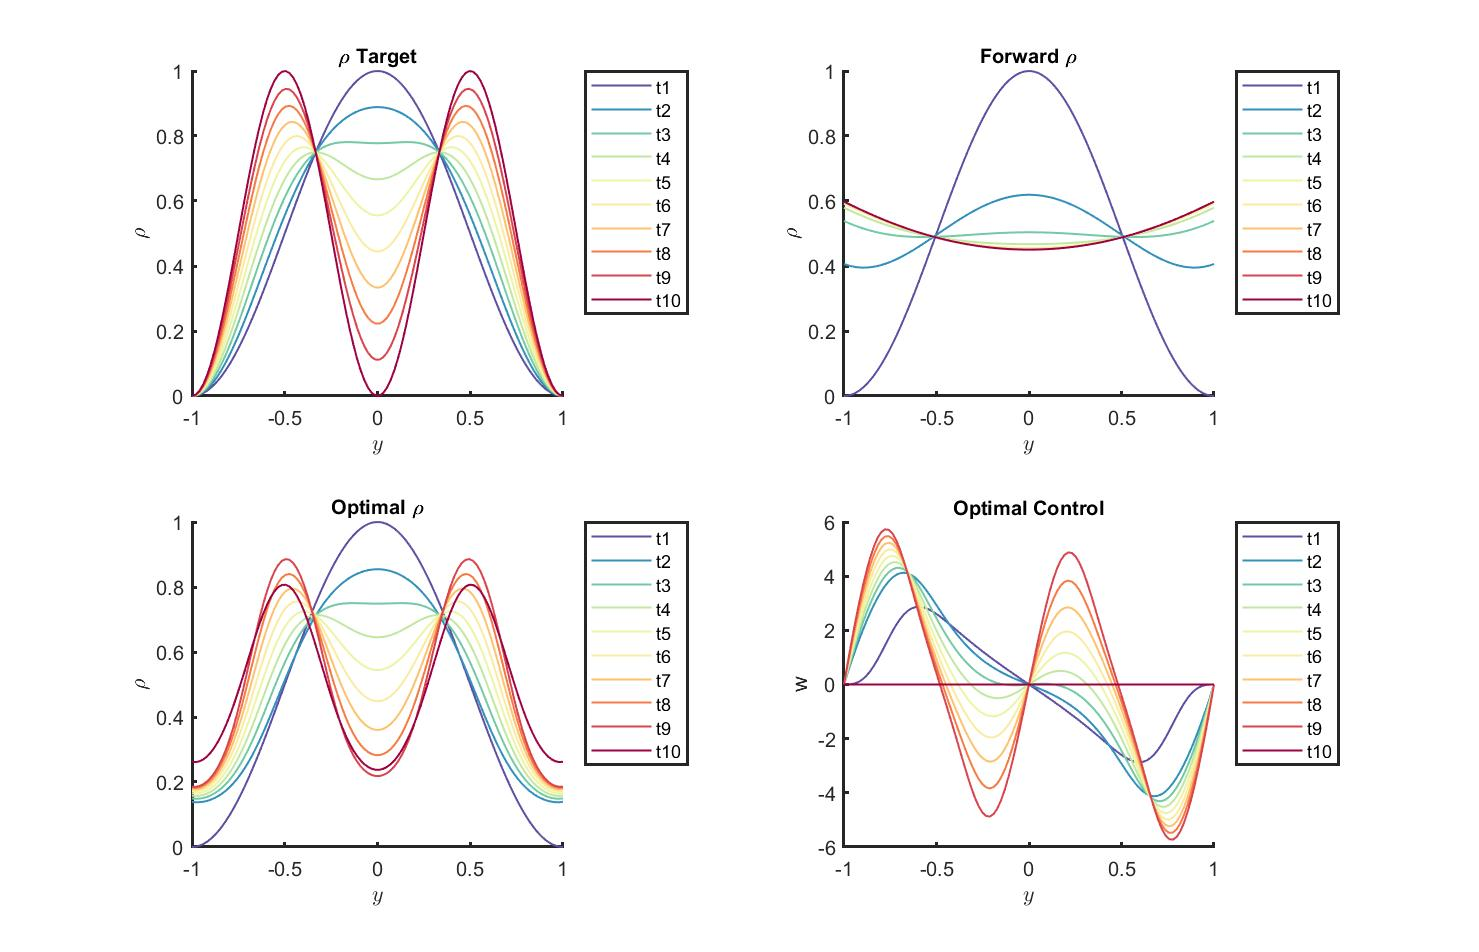
\includegraphics[scale=0.3]{Res2Peak2b.jpg}
	\caption{Results for Neumann Flow, $2$ Peak Example $2$, $\gamma = 1$.}
	\label{Ex12Peak2b}
\end{figure}


\section{Zero-Dirichlet Examples}
We want a Dirichlet example with zero-Dirichlet BCs, $\rho$ of mass $1$ and positive. We can use the same initial condition for $\rho$ and $\hat \rho$ as in the second Neumann example above.
Choose the intital condition:
\begin{align*}
\rho_{IC} = \frac{1}{2}\cos(\pi y) + \frac{1}{2},
\end{align*}
and the target:
\begin{align*}
\hat \rho = \bigg(\frac{1}{2}\cos(\pi y) + \frac{1}{2}\bigg)(1-t) + t\bigg(-\frac{1}{2}\cos(2 \pi y) + \frac{1}{2}\bigg).
\end{align*}
For $\beta = 10^{-3}$, $\gamma = 0$, $J_{FW} = 0.1545$, $J_{Opt} = 0.0380$, see Figure \ref{ResD01}.
\begin{figure}[h]
	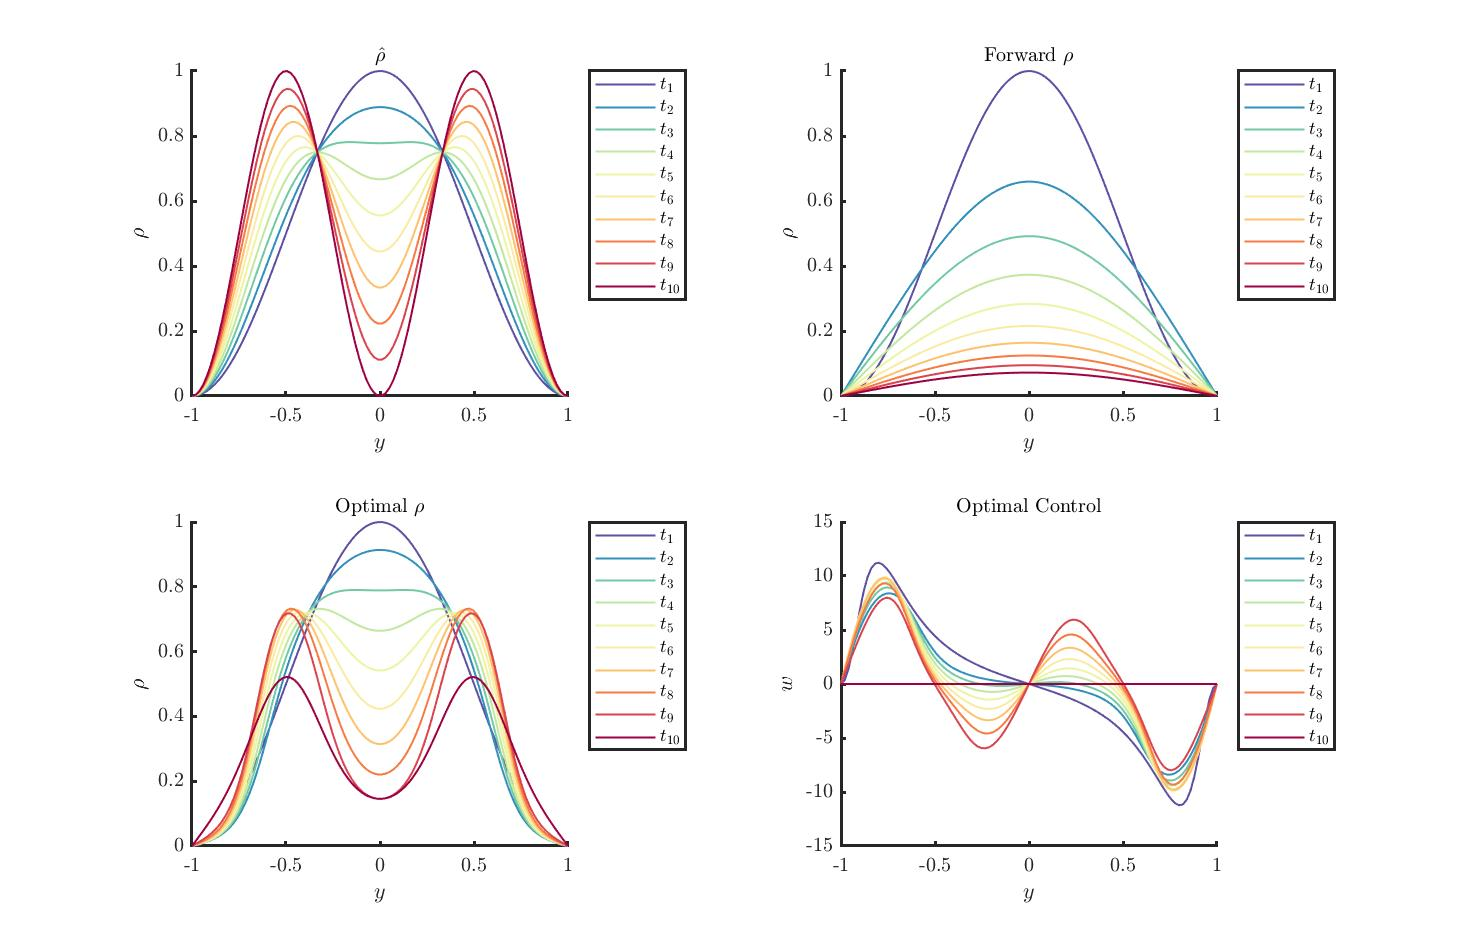
\includegraphics[scale=0.3]{ResD01.jpg}
	\caption{Results for zero-Dirichlet Flow, Example $1$, $\gamma = 0$.}
	\label{ResD01}
\end{figure}
For $\beta = 10^{-3}$, $\gamma = -1$, $J_{FW} = 0.1417$, $J_{Opt} = 0.0356$, see Figure \ref{ResD01a}.
\begin{figure}[h]
	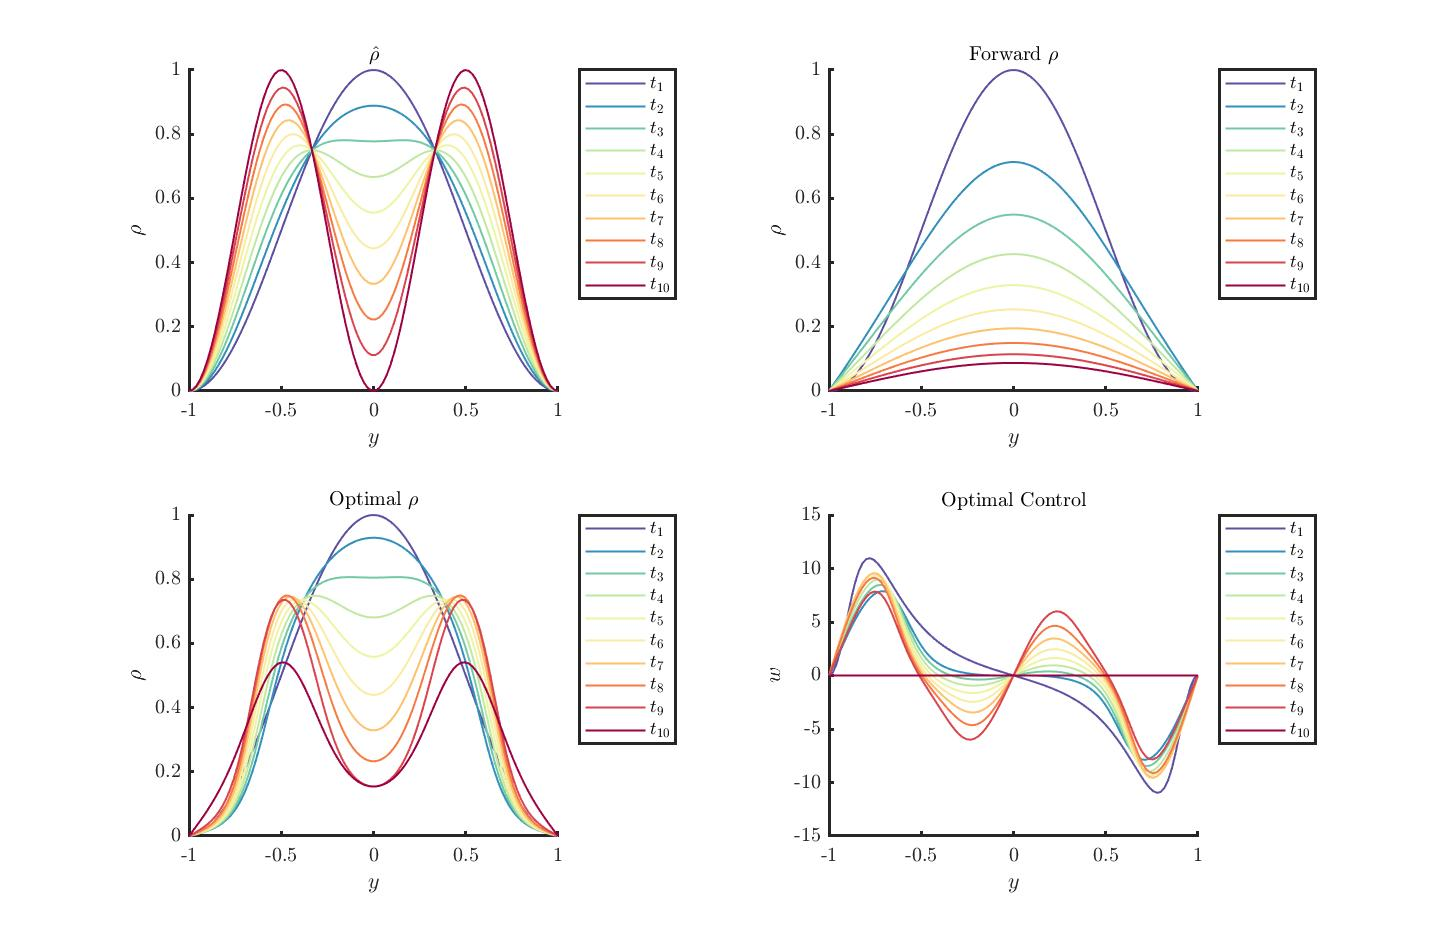
\includegraphics[scale=0.3]{ResD01a.jpg}
	\caption{Results for zero-Dirichlet Flow, Example $1$, $\gamma = -1$.}
	\label{ResD01a}
\end{figure}
For $\beta = 10^{-3}$, $\gamma = 1$, $J_{FW} = 0.1661$, $J_{Opt} = 0.0411$, see Figure \ref{ResD01b}.
\begin{figure}[h]
	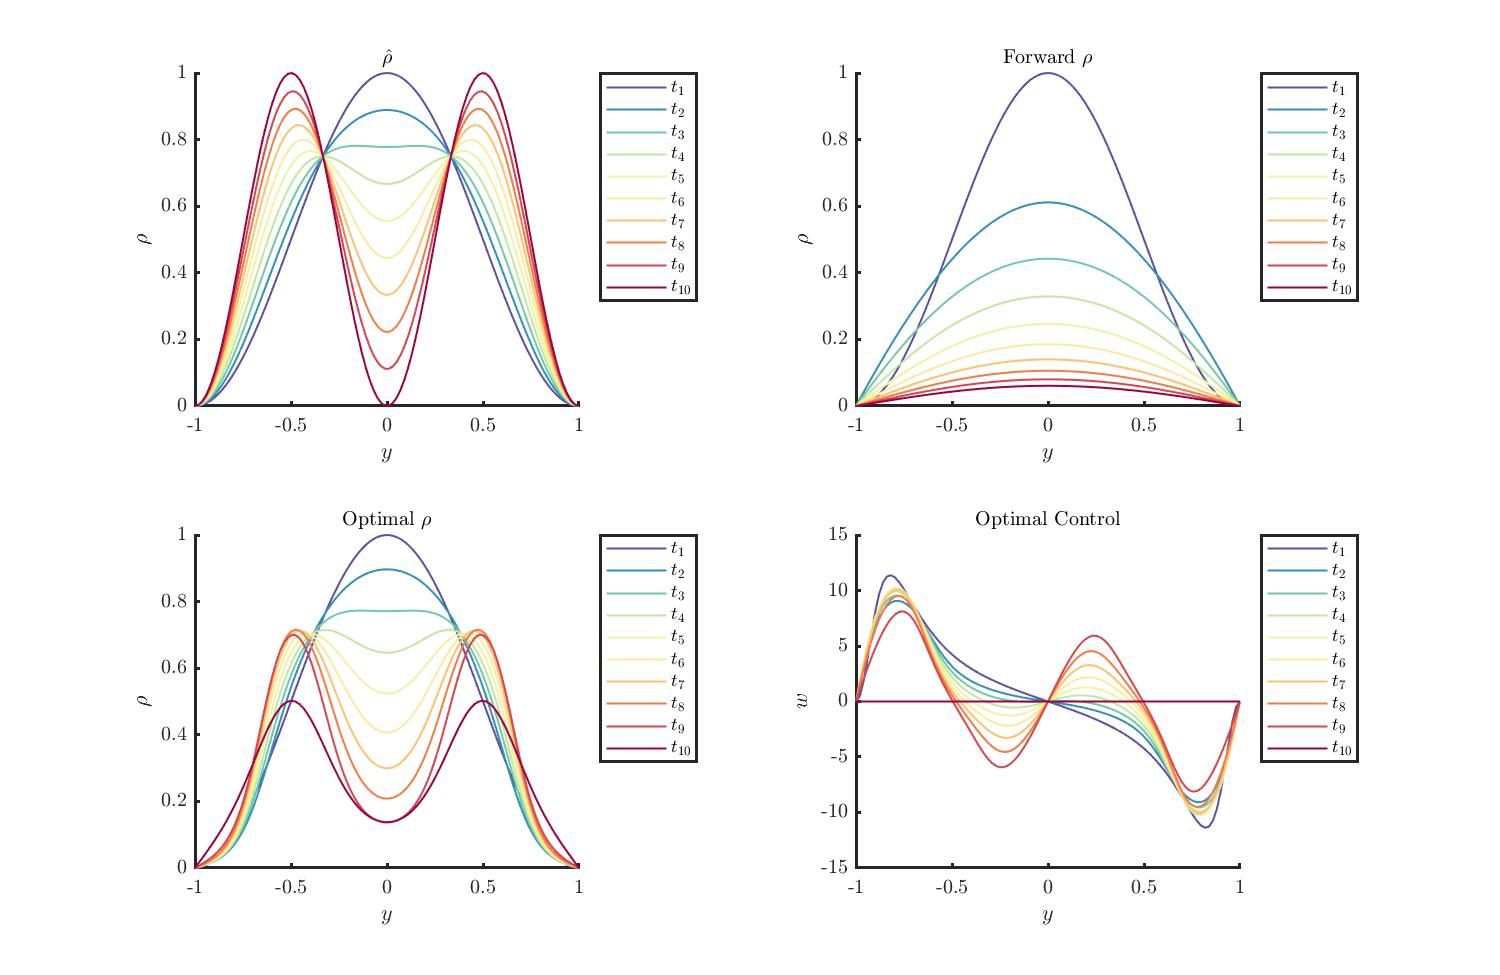
\includegraphics[scale=0.3]{ResD01b.jpg}
	\caption{Results for zero-Dirichlet Flow, Example $1$, $\gamma = 1$.}
	\label{ResD01b}
\end{figure}
There are only very small differences in the three $\gamma$ values.



\section{Non-zero Dirichlet Examples}
Wrong $p$ before. Open question: why did it still work?\\
Now $p$ has zero-Dirichlet conditions and zero final time condition.
\subsection{Example 1}
We have a constant initial condition:
\begin{align*}
\rho_{IC} = 0.5,
\end{align*}
and the target is:
\begin{align*}
\hat \rho = 0.5(1-t) + t(-\frac{1}{4}\cos(\pi y) + \frac{1}{4}).
\end{align*}
For $\beta = 10^{-3}$, $\gamma = 0$, $J_{FW} = 0.0313$, $J_{Opt} = 0.0018$, see Figure \ref{Res1D05}.
\begin{figure}[h]
	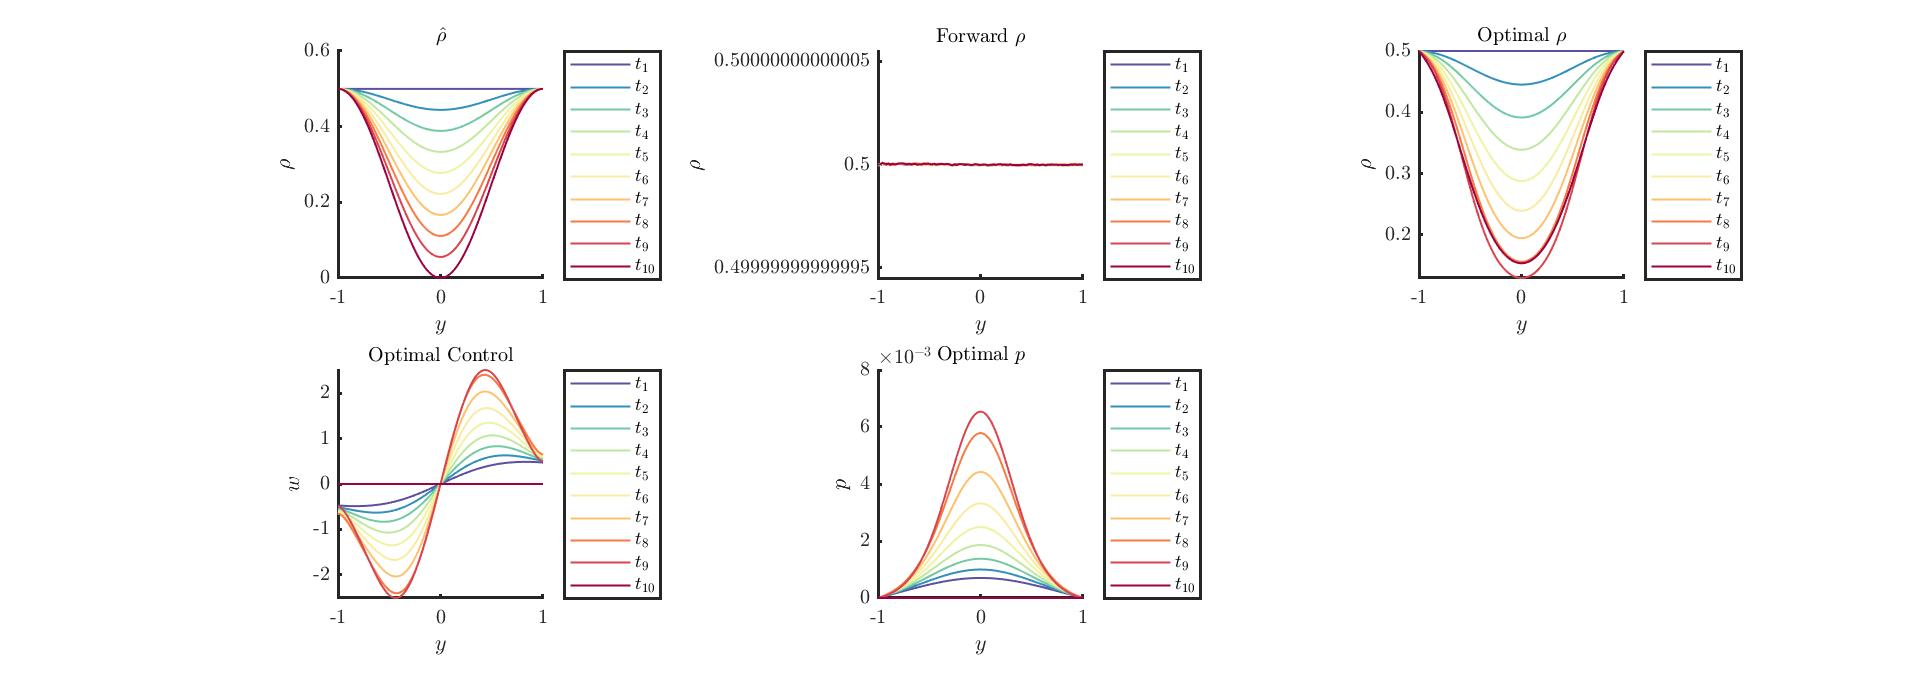
\includegraphics[scale=0.3]{ResD051.jpg}
	\caption{Results for non-zero Dirichlet Flow, Example $1$, $\gamma = 0$.}
	\label{Res1D05}
\end{figure}
For $\beta = 10^{-3}$, $\gamma = -1$, $J_{FW} = 0.0741$, $J_{Opt} = 0.0022$, see Figure \ref{Res1aD05}.
\begin{figure}[h]
	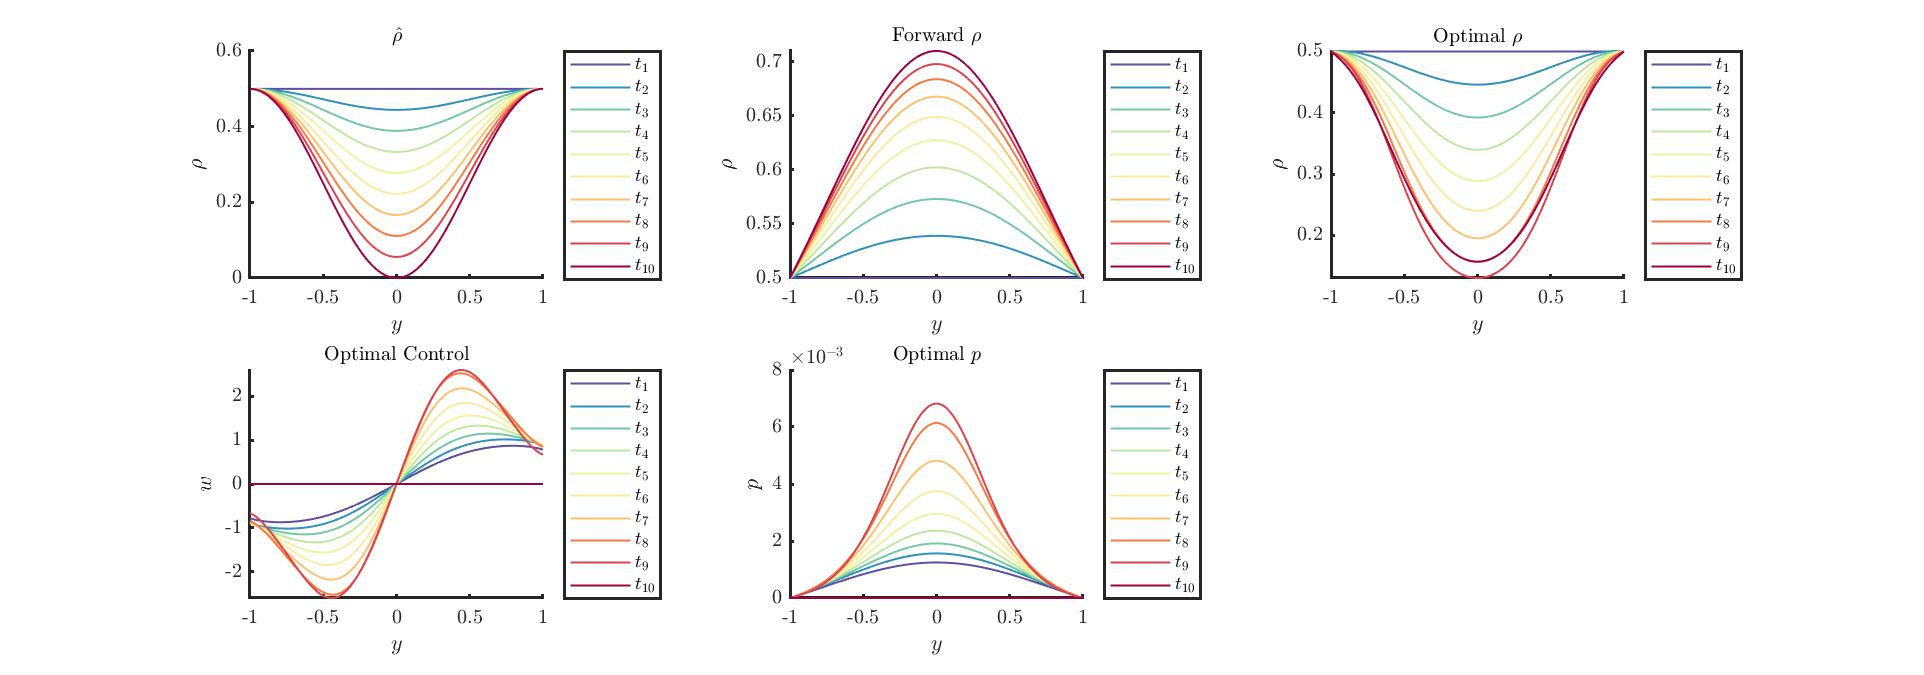
\includegraphics[scale=0.3]{ResD051a.jpg}
	\caption{Results for non-zero Dirichlet Flow, Example $1$, $\gamma = -1$.}
	\label{Res1aD05}
\end{figure}
For $\beta = 10^{-3}$, $\gamma = 1$, $J_{FW} = 0.0148$, $J_{Opt} = 0.0015$, see Figure \ref{Res1bD05}.
\begin{figure}[h]
	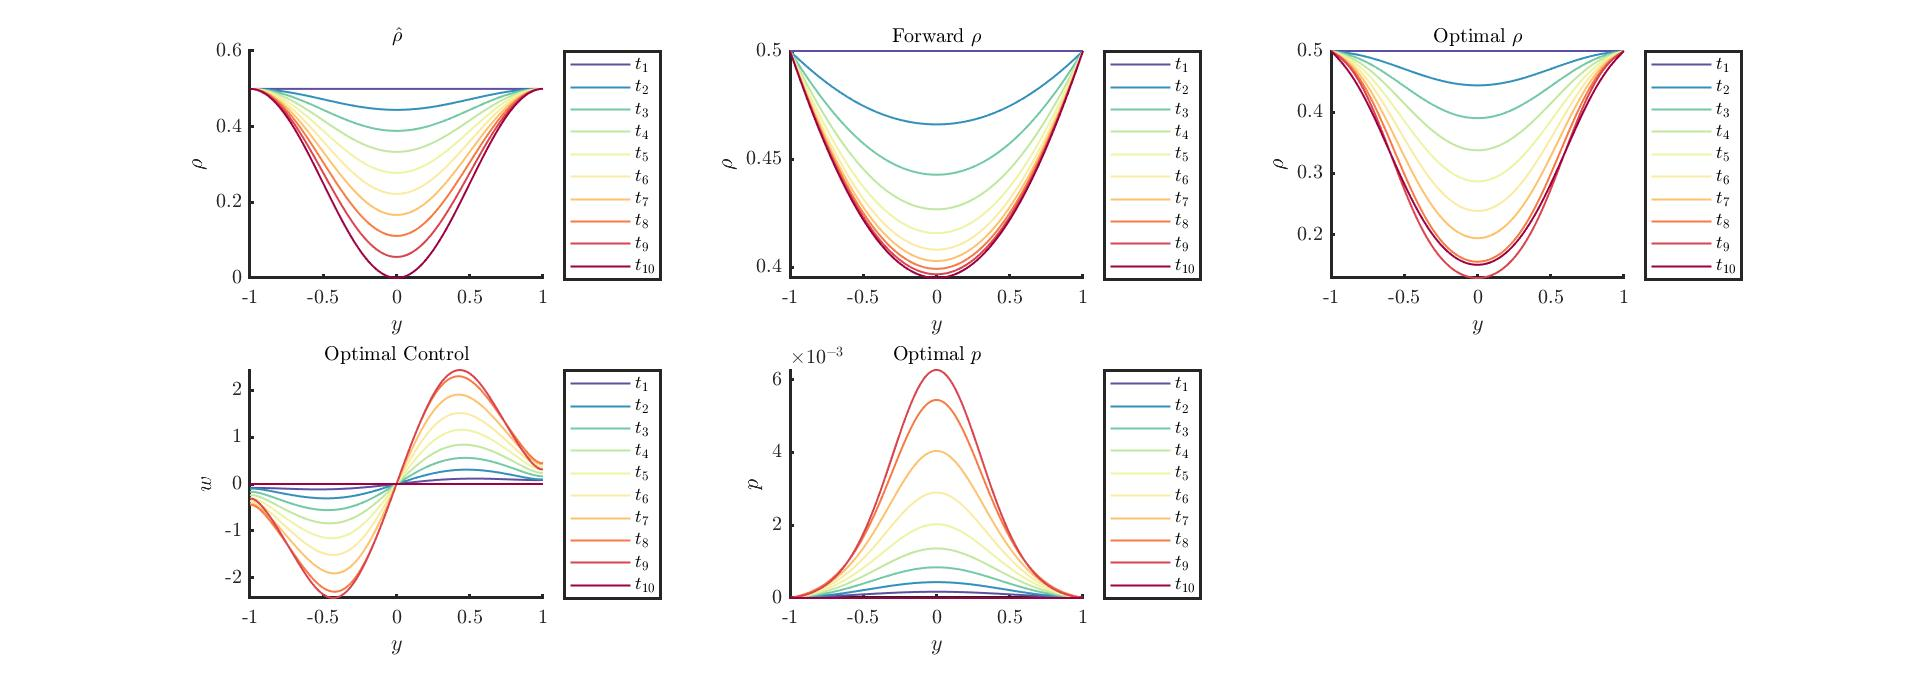
\includegraphics[scale=0.3]{ResD051b.jpg}
	\caption{Results for non-zero Dirichlet Flow, Example $1$, $\gamma = 1$.}
	\label{Res1bD05}
\end{figure}
While the results for $\gamma =0$ and $\gamma = -1$ are similar, $\gamma = 1$ shows a difference in the Optimal Control.

\subsection{Example 2}
We have a constant initial condition 
\begin{align*}
\rho_{IC}= 0.5,
\end{align*}
and the target is:
\begin{align*}
\hat \rho = 0.5(1-t) + t(\frac{1}{2}(\sin(\pi y ) +1)).
\end{align*}
For $\beta = 10^{-3}$, $\gamma = 0$, $J_{FW} = 0.0417$, $J_{Opt} = 0.0027$, see Figure \ref{Res2D05}.
\begin{figure}[h]
	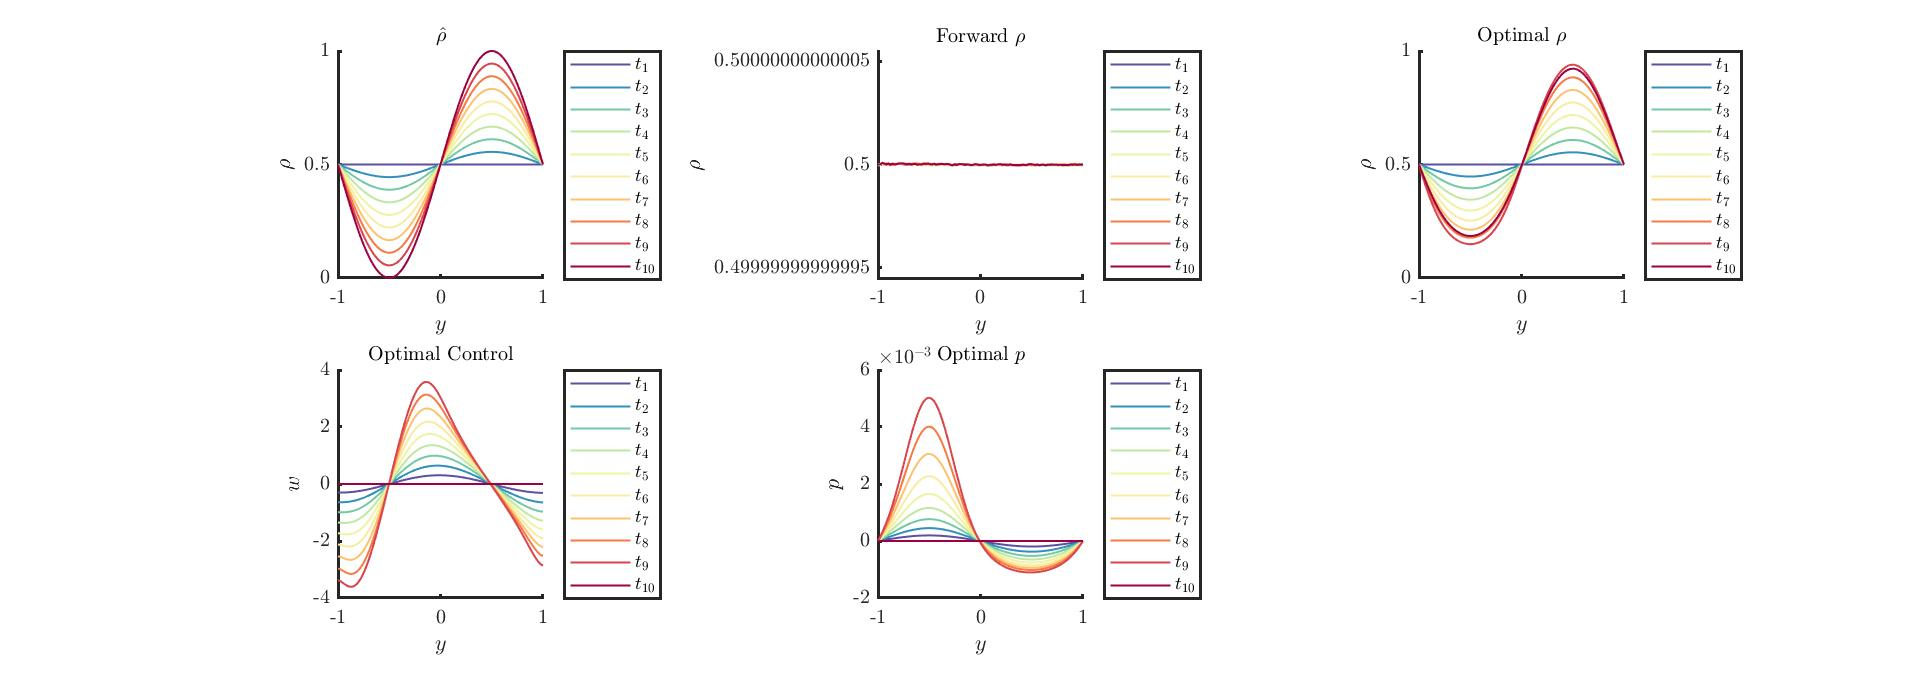
\includegraphics[scale=0.3]{ResD052.jpg}
	\caption{Results for non-zero Dirichlet Flow, Example $2$, $\gamma = 0$.}
	\label{Res2D05}
\end{figure}
For $\beta = 10^{-3}$, $\gamma = -1$, $J_{FW} = 0.0510$, $J_{Opt} = 0.0026$, see Figure \ref{Res2aD05}.
\begin{figure}[h]
	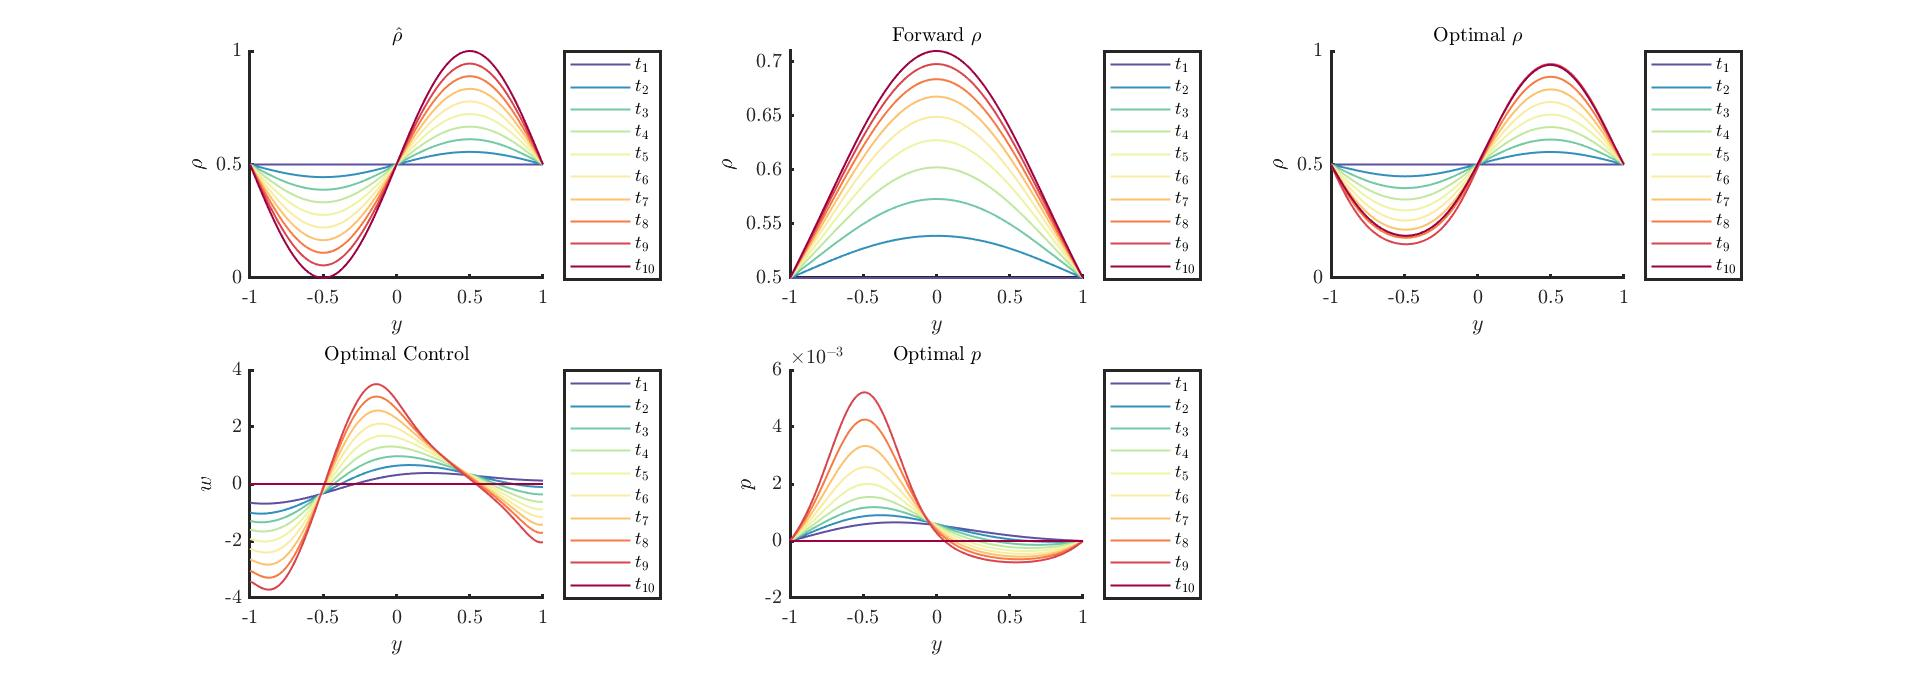
\includegraphics[scale=0.3]{ResD052a.jpg}
	\caption{Results for non-zero Dirichlet Flow, Example $2$, $\gamma = -1$.}
	\label{Res2aD05}
\end{figure}
For $\beta = 10^{-3}$, $\gamma = 1$, $J_{FW} = 0.0452$, $J_{Opt} = 0.0030$, see Figure \ref{Res2bD05}.
\begin{figure}[h]
	\includegraphics[scale=0.3]{ResD052b.jpg}
	\caption{Results for non-zero Dirichlet Flow, Example $2$, $\gamma = 1$.}
	\label{Res2bD05}
\end{figure}
While the examples are again very similar, there are differences to be seen in the Optimal Control.


\subsection{Example 3}
This example is just the reflection of Example 2 (in $\hat \rho$). We have a constant initial condition 
\begin{align*}
\rho_{IC}= 0.5,
\end{align*}
and the target is:
\begin{align*}
\hat \rho = 0.5(1-t) + t(\frac{1}{2}(-\sin(\pi y ) +1)).
\end{align*}
For $\beta = 10^{-3}$, $\gamma = 0$, $J_{FW} = 0.0417$, $J_{Opt} = 0.0027$, see Figure \ref{Res3D05}.
\begin{figure}[h]
	\includegraphics[scale=0.3]{ResD053.jpg}
	\caption{Results for non-zero Dirichlet Flow, Example $3$, $\gamma = 0$.}
	\label{Res3D05}
\end{figure}
For $\beta = 10^{-3}$, $\gamma = -1$, $J_{FW} = 0.0510$, $J_{Opt} = 0.0026$, see Figure \ref{Res3aD05}.
\begin{figure}[h]
	\includegraphics[scale=0.3]{ResD053a.jpg}
	\caption{Results for non-zero Dirichlet Flow, Example $3$, $\gamma = -1$.}
	\label{Res3aD05}
\end{figure}
For $\beta = 10^{-3}$, $\gamma = 1$, $J_{FW} = 0.0452$, $J_{Opt} = 0.0030$, see Figure \ref{Res3bD05}.
\begin{figure}[h]
	\includegraphics[scale=0.3]{ResD053b.jpg}
	\caption{Results for non-zero Dirichlet Flow, Example $3$, $\gamma = 1$.}
	\label{Res3bD05}
\end{figure}
Since this is the reflection of Example 2, the values of the cost functional are the same and the Figures show the same qualitative differences for different interactions.

\section{Force Control Examples}

\subsection{Dirichlet}
The initial condition for $\rho$ is 
\begin{align*}
\rho_{IC} = \frac{1}{2}\cos(\pi y) + \frac{1}{2},
\end{align*}
the target is
\begin{align*}
\hat \rho = (1 - t)\frac{1}{2}\cos(\pi y) + \frac{1}{2}  + t\bigg(-\frac{1}{2}\cos(\pi y) + \frac{1}{2}\bigg).
\end{align*}
For $\beta = 10^{-3}$, $\gamma = 0$, $J_{FW} = 0.1545$, $J_{Opt} = 0.0200$, see Figure \ref{ResFD1}.
\begin{figure}[h]
	\includegraphics[scale=0.3]{ResFD1.jpg}
	\caption{Results for Dirichlet Force Control, $\gamma = 0$.}
	\label{ResFD1}
\end{figure}
For $\beta = 10^{-3}$, $\gamma = -1$, $J_{FW} = 0.1417$, $J_{Opt} = 0.0203$, see Figure \ref{ResFD1a}.
\begin{figure}[h]
	\includegraphics[scale=0.3]{ResFD1a.jpg}
	\caption{Results for Dirichlet Force Control, $\gamma = -1$.}
	\label{ResFD1a}
\end{figure}
For $\beta = 10^{-3}$, $\gamma = 1$, $J_{FW} = 0.1661$, $J_{Opt} = 0.0205$, see Figure \ref{ResFD1b}.
\begin{figure}[h]
	\includegraphics[scale=0.3]{ResFD1b.jpg}
	\caption{Results for Dirichlet Force Control, $\gamma = 1$.}
	\label{ResFD1b}
\end{figure}
Small differences can be seen for the different interaction strengths but nothing extreme.

\subsection{Neumann}
Note, different to the other above cases, Neumann Force Control needs a smaller $\lambda$ value of $0.001$ instead of $0.01$.

The initial condition for $\rho$ is 
\begin{align*}
\rho_{IC} = 0.5,
\end{align*}
the target is
\begin{align*}
\hat \rho = 0.5(1-t) + t\frac{1}{2}(-\cos(\pi y) + 1).
\end{align*}
For $\beta = 10^{-3}$, $\gamma = 0$, $J_{FW} = 0.0417$, $J_{Opt} = 0.0045$, see Figure \ref{ResFN1}.
\begin{figure}[h]
	\includegraphics[scale=0.3]{ResFN1.jpg}
	\caption{Results for Neumann Force Control, $\gamma = 0$.}
	\label{ResFN1}
\end{figure}
For $\beta = 10^{-3}$, $\gamma = -1$, $J_{FW} = 0.0606$, $J_{Opt} = 0.0060$, see Figure \ref{ResFN1a}.
\begin{figure}[h]
	\includegraphics[scale=0.3]{ResFN1a.jpg}
	\caption{Results for Neumann Force Control, $\gamma = -1$.}
	\label{ResFN1a}
\end{figure}
For $\beta = 10^{-3}$, $\gamma = 1$, $J_{FW} = 0.0286$, $J_{Opt} = 0.0036$, see Figure \ref{ResFN1b}.
\begin{figure}[h]
	\includegraphics[scale=0.3]{ResFN1b.jpg}
	\caption{Results for Neumann Force Control, $\gamma = 1$.}
	\label{ResFN1b}
\end{figure}
There are some differences in the optimal control for the different interaction strengths, but not too big ones.





\end{document}